% !TeX spellcheck = hu_HU
% !TeX encoding = UTF-8
% !TeX program = xelatex
\documentclass[12pt,a4paper,oneside]{report}

% thanks to http://tex.stackexchange.com/a/47579/71109
\usepackage{ifxetex}
\usepackage{ifluatex}
\newif\ifxetexorluatex % a new conditional starts as false
\ifnum 0\ifxetex 1\fi\ifluatex 1\fi>0
  \xetexorluatextrue
\fi

\ifxetexorluatex
  \usepackage{fontspec}
\else
  \usepackage[T1]{fontenc}
  \usepackage[utf8]{inputenc}
  \usepackage[lighttt]{lmodern}
\fi

\usepackage[english,magyar]{babel} % Alapértelmezés szerint utoljára definiált nyelv lesz aktív, de később külön beállítjuk az aktív nyelvet.

%\usepackage{cmap}
\usepackage{amsfonts,amsmath,amssymb} % Mathematical symbols.
%\usepackage[ruled,boxed,resetcount,linesnumbered]{algorithm2e} % For pseudocodes. % beware: this is not compatible with LuaLaTeX, see http://tex.stackexchange.com/questions/34814/lualatex-and-algorithm2e
\usepackage{booktabs} % For publication quality tables for LaTeX
\usepackage{graphicx}

%\usepackage{fancyhdr}
%\usepackage{lastpage}

\usepackage{anysize}
%\usepackage{sectsty}
\usepackage{setspace} % For setting line spacing

\usepackage[unicode]{hyperref} % For hyperlinks in the generated document.
\usepackage{xcolor}
\usepackage{listings} % For source code snippets.

\usepackage[amsmath,thmmarks]{ntheorem} % Theorem-like environments.

\usepackage[hang]{caption}

\newcommand{\selecthungarian}{
  \selectlanguage{magyar}
  \setlength{\parindent}{2em}
  \setlength{\parskip}{0em}
  \frenchspacing
}

\newcommand{\selectenglish}{
  \selectlanguage{english}
  \setlength{\parindent}{0em}
  \setlength{\parskip}{0.5em}
  \nonfrenchspacing
  \renewcommand{\figureautorefname}{Figure}
  \renewcommand{\tableautorefname}{Table}
  \renewcommand{\partautorefname}{Part}
  \renewcommand{\chapterautorefname}{Chapter}
  \renewcommand{\sectionautorefname}{Section}
  \renewcommand{\subsectionautorefname}{Section}
  \renewcommand{\subsubsectionautorefname}{Section}
}

\usepackage[numbers]{natbib}
\usepackage{xspace}

\usepackage{xurl} % For breaking long URLs in the bibliography.

% js listing
\usepackage{listings}
\usepackage[many]{tcolorbox}
\usepackage{xcolor}

% colors
\definecolor{white}{rgb}{1,1,1}
\definecolor{black}{rgb}{0,0,0}
\definecolor{middlegray}{rgb}{0.5,0.5,0.5}
\definecolor{lightgray}{rgb}{.95,.95,.95}
\definecolor{arsenic}{rgb}{0.23, 0.27, 0.29}
\definecolor{arsenicLight}{rgb}{0.20, 0.20, 0.20}
\definecolor{darkgray}{rgb}{.4,.4,.4}
\definecolor{purple}{rgb}{0.65, 0.12, 0.82}
\definecolor{orange}{rgb}{0.8,0.3,0.3}
\definecolor{yac}{rgb}{0.6,0.6,0.1}
\definecolor{green}{rgb}{.2,0.6,0.3}
\definecolor{azure}{rgb}{0.0, 0.5, 1.0}
\definecolor{editorGray}{rgb}{0.95, 0.95, 0.95}
\definecolor{editorOcher}{rgb}{1, 0.5, 0}
\definecolor{editorGreen}{rgb}{0, 0.5, 0}
\definecolor{orange}{rgb}{1,0.45,0.13}
\definecolor{olive}{rgb}{0.17,0.59,0.20}
\definecolor{brown}{rgb}{0.69,0.31,0.31}
\definecolor{purple}{rgb}{0.38,0.18,0.81}
\definecolor{lightblue}{rgb}{0.1,0.57,0.7}
\definecolor{lightred}{rgb}{1,0.4,0.5}
\definecolor{amber}{rgb}{1.0, 0.75, 0.0}

\definecolor{vscodered}{HTML}{E53935}
\definecolor{vscodelightred}{HTML}{EF5350}
\definecolor{vscodeblue}{HTML}{1565C0}
\definecolor{vscodegreen}{HTML}{66BB6A}

\definecolor{lightblack}{HTML}{212121}
\definecolor{darkraspberry}{rgb}{0.53, 0.15, 0.34}

% blue hues
\definecolor{bleudefrance}{rgb}{0.19, 0.55, 0.91}
\definecolor{brandeisblue}{rgb}{0.0, 0.44, 1.0}
\definecolor{blue(ncs)}{rgb}{0.0, 0.53, 0.74}
\definecolor{coolblack}{rgb}{0.0, 0.18, 0.39}

% red hues
\definecolor{coralred}{rgb}{1.0, 0.25, 0.25}
\definecolor{darkred}{rgb}{0.55, 0.0, 0.0}

% general settings for listing
\lstset{
basicstyle=\normalsize\ttfamily,
basewidth  = {.5em,0.4em},
captionpos=t,
lineskip={2pt},
backgroundcolor=\color{white},
framextopmargin=6pt,
framexrightmargin=0.9em,
framexleftmargin=0.9em,
framexbottommargin=6pt,
frame=tb,
framerule=0pt,
framesep=6.5mm,
fillcolor=\color{white},
rulecolor=\color{middlegray},
numbers=left,
numberstyle=\normalfont\color{middlegray},
numbersep=16pt,
abovecaptionskip=-5pt, %space above the caption
belowcaptionskip=10pt, %space below the caption
extendedchars=true,
showstringspaces=false,
showspaces=false,
stepnumber=1, % the step between two line-numbers. If it is 1 each line will be numbered
tabsize=2,
breaklines=true,
showtabs=false,
upquote=true,
% German umlauts
literate=%
  {Ö}{{\"O}}1
{Ä}{{\"A}}1
{Ü}{{\"U}}1
{ß}{{\ss}}1
{ü}{{\"u}}1
{ä}{{\"a}}1
{ö}{{\"o}}1
}

% define language
\lstdefinelanguage{JavaScript}{
  keywords={typeof, new, true, false, catch, then, function, return, catch, switch, var, if, in, while, do, else, case, break, default, this, process},
  keywordstyle=\color{editorGreen}\bfseries,
  ndkeywords={class, export, boolean, throw, implements, import, from, const, async, await, private, public, readonly, static, constructor, get, set, yield, interface, type},
  ndkeywordstyle=\color{vscodeblue}\bfseries,
  identifierstyle=\color{black},
  sensitive=false,
  comment=[l]{//},
  morecomment=[s]{/*}{*/},
  commentstyle=\color{editorGreen}\ttfamily,
  stringstyle=\color{darkred}\ttfamily,
  morestring=[b]',
  morestring=[b]",
  morestring=*[d]`,
  moredelim=[s][]{\$\{}{\}},
  morekeywords=[3]{@UseGuards, @ApiFoundResponse, @ApiQuery, @Controller, @Injectable, @Module, @Inject, @Body, @Param, @Query, @UseInterceptors, @UseFilters, @UploadedFile, @UsePipes, @Get, @Post, @Put, @Delete, @Patch, @CurrentUser, @Res, @Next, @Headers, @Session, @Request, @All, string, number, null, void, undefined},
  keywordstyle={[3]\color{darkraspberry}\bfseries}
}

\lstdefinelanguage{SQL}{
  keywords={select, where, from},
  keywordstyle=\color{editorGreen}\bfseries,
  ndkeywords={},
  ndkeywordstyle=\color{vscodeblue}\bfseries,
  identifierstyle=\color{black},
  sensitive=false,
  comment=[l]{--},
  morecomment=[s]{/*}{*/},
  commentstyle=\color{editorGreen}\ttfamily,
  stringstyle=\color{darkred}\ttfamily,
  morestring=[b]',
  morestring=[b]"
}


\lstdefinelanguage{HTML5}{
  language=html,
  sensitive=true,
  alsoletter={<>=-},
  morecomment=[s]{<!-}{-->},
  tag=[s],
  otherkeywords={
      % General
      >,
      % Standard tags
      <!DOCTYPE,
      </html, <html, <head, <title, </title, <style, </style, <link, </head, <meta, />,
      % body
      </body, <body,
      % Divs
      </div, <div, </div>,
      % Paragraphs
      </p, <p, </p>,
      % scripts
      </script, <script,
      % More tags...
      <canvas, /canvas>, <svg, <rect, <animateTransform, </rect>, </svg>, <video, <source, <iframe, </iframe>, </video>, <image, </image>, <header, </header, <article, </article
    },
  ndkeywords={
      % General
      =,
      % HTML attributes
      charset=, src=, id=, width=, height=, style=, type=, rel=, href=,
      % SVG attributes
      fill=, attributeName=, begin=, dur=, from=, to=, poster=, controls=, x=, y=, repeatCount=, xlink:href=,
      % properties
      margin:, padding:, background-image:, border:, top:, left:, position:, width:, height:, margin-top:, margin-bottom:, font-size:, line-height:,
      % CSS3 properties
      transform:, -moz-transform:, -webkit-transform:,
      animation:, -webkit-animation:,
      transition:,  transition-duration:, transition-property:, transition-timing-function:,
    }
}

\lstdefinelanguage{Terraform}{
  keywords={terraform, variable, locals, output, module, resource, data, backend, true, false, var, local},
  keywordstyle=\color{vscodegreen}\bfseries,
  ndkeywords={lifecycle, provisioner, connection, length, lookup, merge, coalesce, zipmap, flatten, try, null, for, if, else, each, in, template_file, object, map, string, number, null_resource},
  ndkeywordstyle=\color{vscodeblue}\bfseries,
  sensitive=false,
  comment=[l]{\#},
  commentstyle=\color{editorGreen}\ttfamily,
  stringstyle=\color{darkred}\ttfamily,
  moredelim=[s][]{\$\{}{\}},
  morestring=[b]',
  morestring=*[d]",
  identifierstyle=\color{black}\ttfamily,
}

\lstdefinelanguage{Dockerfile}{
  keywords={FROM, RUN, COPY, ADD, ENTRYPOINT, CMD,  ENV, ARG, WORKDIR, EXPOSE, LABEL, USER, VOLUME, STOPSIGNAL, ONBUILD, MAINTAINER, HEALTHCHECK},
  keywordstyle=\color{vscodeblue}\bfseries,
  identifierstyle=\color{black},
  sensitive=false,
  comment=[l]{\#},
  commentstyle=\color{editorGreen}\ttfamily,
  stringstyle=\color{darkred}\ttfamily,
  morestring=[b]',
  morestring=[b]"
}

\lstdefinestyle{html} {%
% Code design
keywordstyle=\color{lightblack}\bfseries,
ndkeywordstyle=\color{lightblack}\bfseries,
identifierstyle=\color{lightblack},
commentstyle=\color{green}\ttfamily,
stringstyle=\color{darkred}\ttfamily,
% Code
language=HTML5,
%  alsolanguage=JavaScript,
alsodigit={.:;},
tabsize=2,
showtabs=false,
showspaces=false,
showstringspaces=false,
extendedchars=true,
breaklines=true,
% German umlauts
literate=%
  {Ö}{{\"O}}1
{Ä}{{\"A}}1
{Ü}{{\"U}}1
{ß}{{\ss}}1
{ü}{{\"u}}1
{ä}{{\"a}}1
{ö}{{\"o}}1
}

\lstdefinelanguage{CSS}
{morekeywords={color,background,margin,padding,margin,padding,font,weight,display,position,top,left,right,bottom,list,style,border,size,white,space,min,width, 	transition},
  sensitive=false,
  morecomment=[l]{//},
  morecomment=[s]{/*}{*/},
  morestring=[b]",
}

\newcommand\YAMLcolonstyle{\color{darkred}\mdseries}
\newcommand\YAMLkeystyle{\color{black}\bfseries}
\newcommand\YAMLvaluestyle{\color{vscodeblue}\mdseries}

\lstdefinelanguage{YAML}{
  keywords={true,false,null,y,n},
  keywordstyle=\color{darkgray}\bfseries,
  basicstyle=\YAMLkeystyle,                                 % assuming a key comes first
  sensitive=false,
  comment=[l]{\#},
  morecomment=[s]{/*}{*/},
  commentstyle=\color{editorGreen}\ttfamily,
  stringstyle=\YAMLvaluestyle\ttfamily,
  % moredelim=[l][\color{orange}]{\&},
  moredelim=[l][\color{magenta}]{*},
  moredelim=**[il][\YAMLcolonstyle{:}\YAMLvaluestyle]{:},   % switch to value style at :
  morestring=[b]',
  morestring=[b]",
  literate =    {---}{{\ProcessThreeDashes}}3
  {>}{{\textcolor{red}\textgreater}}1
  {|}{{\textcolor{red}\textbar}}1
  {\ -\ }{{\mdseries\ -\ }}3,
}

\lstdefinestyle{css} {
  language=CSS,
  keywordstyle=\color{lightblack},
}

\lstdefinestyle{js} {
  language=JavaScript
}

\lstdefinestyle{tf} {
  language=Terraform
}

\lstdefinestyle{dockerfile} {
  language=Dockerfile
}

\lstdefinestyle{yaml} {
  language=YAML
}

\lstdefinestyle{sql} {
  language=SQL,
  keywordstyle=\color{azure}
}

% Hyphenation rules
\hyphenation{PostgreSQL Cloud-Front strea-ming stream pa-cket Apple Lambda Edge Route Node Vite Actions Action Type-Script Java-Script-ből Java-Script React Function Rou-ter route table build buil-del Re-quest bucket re-po-si-to-ry Docker Registry Se-cu-ri-ty Group Gate-way Cloud-Watch AuthSCH OAuth Chrome Google Media-Package Media-Live back-end front-end}


\onehalfspacing % Set line spacing to 1.5

\newcommand{\vikszerzoVezeteknev}{Piller}
\newcommand{\vikszerzoKeresztnev}{Trisztán}

\newcommand{\vikkonzulensAMegszolitas}{}
\newcommand{\vikkonzulensAVezeteknev}{Kövesdán}
\newcommand{\vikkonzulensAKeresztnev}{Gábor}

\newcommand{\vikkonzulensBMegszolitas}{}
\newcommand{\vikkonzulensBVezeteknev}{}
\newcommand{\vikkonzulensBKeresztnev}{}

\newcommand{\vikkonzulensCMegszolitas}{}
\newcommand{\vikkonzulensCVezeteknev}{}
\newcommand{\vikkonzulensCKeresztnev}{}

\newcommand{\vikcim}{Videó streaming szolgáltatások implementációja}
\newcommand{\viktanszek}{\bmeaut} 
\newcommand{\vikdoktipus}{\msc}
\newcommand{\vikmunkatipusat}{diplomatervet} 

%--------------------------------------------------------------------------------------
% TDK-specifikus változók
%--------------------------------------------------------------------------------------
\newcommand{\tdkszerzoB}{Második Szerző} % Második szerző neve; hagyd üresen, ha egyedül írtad a TDK-t.
\newcommand{\tdkev}{2014} % A dolgozat írásának éve (pl. "2014") (Ez OTDK-nál eltérhet az aktuális évtől.)

% További adatok az OTDK címlaphoz (BME-s TDK-hoz nem kell kitölteni)
\newcommand{\tdkevfolyamA}{IV} % Első szerző évfolyama, római számmal (pl. IV).
\newcommand{\tdkevfolyamB}{III} % Második szerző évfolyama, római számmal (pl. III).
\newcommand{\tdkkonzulensbeosztasA}{egyetemi tanár} % Első konzulens beosztása (pl. egyetemi docens)
\newcommand{\tdkkonzulensbeosztasB}{doktorandusz} % Második konzulens beosztása (pl. egyetemi docens)

\newcommand{\szerzoMeta}{\vikszerzoVezeteknev{} \vikszerzoKeresztnev} 

%--------------------------------------------------------------------------------------
% Elnevezések
%--------------------------------------------------------------------------------------
\newcommand{\bme}{Budapesti Műszaki és Gazdaságtudományi Egyetem}
\newcommand{\vik}{Villamosmérnöki és Informatikai Kar}

\newcommand{\bmemit}{Méréstechnika és Információs Rendszerek Tanszék}
\newcommand{\bmeaut}{Automatizálási és Alkalmazott Informatikai Tanszék}

\newcommand{\keszitette}{Készítette}
\newcommand{\konzulens}{Konzulens}

\newcommand{\bsc}{Szakdolgozat}
\newcommand{\msc}{Diplomaterv}
\newcommand{\tdk}{TDK dolgozat}
\newcommand{\bsconlab}{BSc Önálló laboratórium}
\newcommand{\msconlabi}{MSc Önálló laboratórium 1.}
\newcommand{\msconlabii}{MSc Önálló laboratórium 2.}

\newcommand{\pelda}{Példa}
\newcommand{\definicio}{Definíció}
\newcommand{\tetel}{Tétel}

\newcommand{\bevezetes}{Bevezetés}
\newcommand{\koszonetnyilvanitas}{Köszönetnyilvánítás}
\newcommand{\fuggelek}{Függelék}

% Opcionálisan átnevezhető címek
%\addto\captionsmagyar{%
%\renewcommand{\listfigurename}{Saját ábrajegyzék cím}
%\renewcommand{\listtablename}{Saját táblázatjegyzék cím}
%\renewcommand{\bibname}{Saját irodalomjegyzék név}
%}

\newcommand{\szerzo}{\vikszerzoVezeteknev{} \vikszerzoKeresztnev}
\newcommand{\vikkonzulensA}{\vikkonzulensAMegszolitas\vikkonzulensAVezeteknev{} \vikkonzulensAKeresztnev}
\newcommand{\vikkonzulensB}{\vikkonzulensBMegszolitas\vikkonzulensBVezeteknev{} \vikkonzulensBKeresztnev}
\newcommand{\vikkonzulensC}{\vikkonzulensCMegszolitas\vikkonzulensCVezeteknev{} \vikkonzulensCKeresztnev}

\newcommand{\selectthesislanguage}{\selecthungarian}

\bibliographystyle{huplain}

\def\lstlistingname{lista}

\newcommand{\appendixnumber}{6}  % a fofejezet-szamlalo az angol ABC 6. betuje (F) lesz

%--------------------------------------------------------------------------------------
% Page layout setup
%--------------------------------------------------------------------------------------
% we need to redefine the pagestyle plain
% another possibility is to use the body of this command without \fancypagestyle
% and use \pagestyle{fancy} but in that case the special pages
% (like the ToC, the References, and the Chapter pages)remain in plane style

\pagestyle{plain}
\marginsize{35mm}{25mm}{15mm}{15mm}

\setcounter{tocdepth}{3}
%\sectionfont{\large\upshape\bfseries}
\setcounter{secnumdepth}{3}

\sloppy % Margón túllógó sorok tiltása.
\widowpenalty=10000 \clubpenalty=10000 %A fattyú- és árvasorok elkerülése
\def\hyph{-\penalty0\hskip0pt\relax} % Kötőjeles szavak elválasztásának engedélyezése


%--------------------------------------------------------------------------------------
% Setup hyperref package
%--------------------------------------------------------------------------------------
\hypersetup{
    % bookmarks=true,            % show bookmarks bar?
    unicode=true,              % non-Latin characters in Acrobat's bookmarks
    pdftitle={\vikcim},        % title
    pdfauthor={\szerzoMeta},    % author
    pdfsubject={\vikdoktipus}, % subject of the document
    pdfcreator={\szerzoMeta},   % creator of the document
    pdfproducer={},    % producer of the document
    pdfkeywords={},    % list of keywords (separate then by comma)
    pdfnewwindow=true,         % links in new window
    colorlinks=true,           % false: boxed links; true: colored links
    linkcolor=black,           % color of internal links
    citecolor=black,           % color of links to bibliography
    filecolor=black,           % color of file links
    urlcolor=black             % color of external links
}


%--------------------------------------------------------------------------------------
% Set up listings
%--------------------------------------------------------------------------------------
\definecolor{lightgray}{rgb}{0.95,0.95,0.95}
\lstset{
	basicstyle=\scriptsize\ttfamily, % print whole listing small
	keywordstyle=\color{black}\bfseries, % bold black keywords
	identifierstyle=, % nothing happens
	% default behavior: comments in italic, to change use
	% commentstyle=\color{green}, % for e.g. green comments
	stringstyle=\scriptsize,
	showstringspaces=false, % no special string spaces
	aboveskip=3pt,
	belowskip=3pt,
	backgroundcolor=\color{lightgray},
	columns=flexible,
	keepspaces=true,
	escapeinside={(*@}{@*)},
	captionpos=b,
	breaklines=true,
	frame=single,
	float=!ht,
	tabsize=2,
	literate=*
		{á}{{\'a}}1	{é}{{\'e}}1	{í}{{\'i}}1	{ó}{{\'o}}1	{ö}{{\"o}}1	{ő}{{\H{o}}}1	{ú}{{\'u}}1	{ü}{{\"u}}1	{ű}{{\H{u}}}1
		{Á}{{\'A}}1	{É}{{\'E}}1	{Í}{{\'I}}1	{Ó}{{\'O}}1	{Ö}{{\"O}}1	{Ő}{{\H{O}}}1	{Ú}{{\'U}}1	{Ü}{{\"U}}1	{Ű}{{\H{U}}}1
}


%--------------------------------------------------------------------------------------
% Set up theorem-like environments
%--------------------------------------------------------------------------------------
% Using ntheorem package -- see http://www.math.washington.edu/tex-archive/macros/latex/contrib/ntheorem/ntheorem.pdf

\theoremstyle{plain}
\theoremseparator{.}
\newtheorem{example}{\pelda}

\theoremseparator{.}
%\theoremprework{\bigskip\hrule\medskip}
%\theorempostwork{\hrule\bigskip}
\theorembodyfont{\upshape}
\theoremsymbol{{\large \ensuremath{\centerdot}}}
\newtheorem{definition}{\definicio}

\theoremseparator{.}
%\theoremprework{\bigskip\hrule\medskip}
%\theorempostwork{\hrule\bigskip}
\newtheorem{theorem}{\tetel}


%--------------------------------------------------------------------------------------
% Some new commands and declarations
%--------------------------------------------------------------------------------------
\newcommand{\code}[1]{{\upshape\ttfamily\scriptsize\indent #1}}
\newcommand{\doi}[1]{DOI: \href{http://dx.doi.org/\detokenize{#1}}{\raggedright{\texttt{\detokenize{#1}}}}} % A hivatkozások közt így könnyebb DOI-t megadni.

\DeclareMathOperator*{\argmax}{arg\,max}
%\DeclareMathOperator*[1]{\floor}{arg\,max}
\DeclareMathOperator{\sign}{sgn}
\DeclareMathOperator{\rot}{rot}


%--------------------------------------------------------------------------------------
% Setup captions
%--------------------------------------------------------------------------------------
\captionsetup[figure]{
	width=.75\textwidth,
	aboveskip=10pt}

\renewcommand{\captionlabelfont}{\bf}
%\renewcommand{\captionfont}{\footnotesize\it}

%--------------------------------------------------------------------------------------
% Hyphenation exceptions
%--------------------------------------------------------------------------------------
\hyphenation{Shakes-peare Mar-seilles ár-víz-tű-rő tü-kör-fú-ró-gép}


\author{\vikszerzo}
\title{\viktitle}

\begin{document}

\pagenumbering{gobble}

% %--------------------------------------------------------------------------------------
% Feladatkiiras (a tanszeken atveheto, kinyomtatott valtozat)
%--------------------------------------------------------------------------------------
\clearpage
\begin{center}
\large
\textbf{FELADATKIÍRÁS}\\
\end{center}

A feladatkiírást a tanszéki adminisztrációban lehet átvenni, és a leadott munkába eredeti, tanszéki pecséttel ellátott és a tanszékvezető által aláírt lapot kell belefűzni (ezen oldal \emph{helyett}, ez az oldal csak útmutatás). Az elektronikusan feltöltött dolgozatban már nem kell beleszerkeszteni ezt a feladatkiírást.


\selectthesislanguage
\hypersetup{pageanchor=false}
%--------------------------------------------------------------------------------------
%	The title page
%--------------------------------------------------------------------------------------
\begin{titlepage}
\begin{center}

\includegraphics[width=60mm,keepaspectratio]{figures/bme_logo.pdf}\\
\vspace{0.3cm}
\textbf{\bme}\\
\textmd{\vik}\\
\textmd{\viktanszek}\\[5cm]

\vspace{0.4cm}
{\huge \bfseries \vikcim}\\[0.8cm]
\vspace{0.5cm}
\textsc{\Large \vikdoktipus}\\[4cm]

{
	\renewcommand{\arraystretch}{0.85}
	\begin{tabular}{cc}
	 \makebox[7cm]{\emph{\keszitette}} & \makebox[7cm]{\emph{\konzulens}} \\ \noalign{\smallskip}
	 \makebox[7cm]{\szerzo} & \makebox[7cm]{\vikkonzulensA} \\
	  & \makebox[7cm]{\vikkonzulensB} \\
	  & \makebox[7cm]{\vikkonzulensC} \\
	\end{tabular}
}

\vfill
{\large \today}
\end{center}
\end{titlepage}
\hypersetup{pageanchor=false}

	
\tableofcontents\vfill

\selectlanguage{magyar}
\pagenumbering{gobble}
%--------------------------------------------------------------------------------------
% Nyilatkozat
%--------------------------------------------------------------------------------------
\begin{center}
\large
\textbf{HALLGATÓI NYILATKOZAT}\\
\end{center}

Alulírott \emph{\vikszerzoVezeteknev{} \vikszerzoKeresztnev}, szigorló hallgató kijelentem, hogy ezt a \vikmunkatipusat{} meg nem engedett segítség nélkül, saját magam készítettem, csak a megadott forrásokat (szakirodalom, eszközök stb.) használtam fel. Minden olyan részt, melyet szó szerint, vagy azonos értelemben, de átfogalmazva más forrásból átvettem, egyértelműen, a forrás megadásával megjelöltem.

Hozzájárulok, hogy a jelen munkám alapadatait (szerző(k), cím, angol és magyar nyelvű tartalmi kivonat, készítés éve, konzulens(ek) neve) a BME VIK nyilvánosan hozzáférhető elektronikus formában, a munka teljes szövegét pedig az egyetem belső hálózatán keresztül (vagy autentikált felhasználók számára) közzétegye. Kijelentem, hogy a benyújtott munka és annak elektronikus verziója megegyezik. Dékáni engedéllyel titkosított diplomatervek esetén a dolgozat szövege csak 3 év eltelte után válik hozzáférhetővé.

\begin{flushleft}
\vspace*{1cm}
Budapest, \today
\end{flushleft}

\begin{flushright}
 \vspace*{1cm}
 \makebox[7cm]{\rule{6cm}{.4pt}}\\
 \makebox[7cm]{\emph{\vikszerzoVezeteknev{} \vikszerzoKeresztnev}}\\
 \makebox[7cm]{hallgató}
\end{flushright}
\thispagestyle{empty}

\vfill
\clearpage
\thispagestyle{empty} % an empty page

\selectthesislanguage

\pagenumbering{roman}
\setcounter{page}{1}

\selecthungarian

%----------------------------------------------------------------------------
% Abstract in Hungarian
%----------------------------------------------------------------------------
\chapter*{Kivonat}\addcontentsline{toc}{chapter}{Kivonat}

Az IT szakma meghatározó kihívása a magasan teljesítőképes, könnyen skálázódó és stabil infrastruktúra létesítése különféle üzleti célok megvalósítására. A hírközlés, a média és a szórakoztatatás iparágaiban is kiemelt figyelmet kap ez a kihívás.

Ezek a virágzó és feltörekvő iparágak folyamatosan igénylik az olyan szoftverfejlesztőket, akik ezekre az iparágakra specializáltan is folyamatosan képzik magukat, valamint mélyen ismerik a szakterület technológiáit.

Diplomatervem célja demonstrálni egy az Amazon Web Services platformján futó felhő alapú médiaszolgáltatás-rendszer alapos tervezésének, implementálásának, valamint tesztelésének folyamatát. A rendszer a videó streaming szolgáltatások területén nyújt weben elérhető megoldást, és a felhasználók számára lehetővé teszi, hogy saját időbeosztásuknak megfelelően férjenek hozzá videótartalmakhoz (Video-on-Demand), valami élő adásokat is tudjanak megtekinteni (live streaming).

A megoldás ismertetése során kiemelt fókuszt kap a komponensek közötti laza kapcsolás kialakítása, az IT biztonsági kockázatok kezelése, az konfigurációmenedzsment fenntarthatósága. Felhasználásra kerülnek modern webes technológiák és DevOps technikák, mint a konténerizáció, a serverless függvények, a CI/CD csővezetékek és az Infrastructure as Code.

\vfill
\selectenglish

%----------------------------------------------------------------------------
% Abstract in English
%----------------------------------------------------------------------------
\chapter*{Abstract}\addcontentsline{toc}{chapter}{Abstract}

A key challenge for the IT profession is to build highly performant, easily scalable and stable infrastructure to support a variety of business goals. This challenge is also a major focus in Telecommunications, also in the Media \& Entertainment industry.

These booming and emerging industries are in constant need of software developers who train themselves continuously for these industries and have a deep knowledge of the technologies in the field.

My thesis project aims to demonstrate the process of thoroughly designing, implementing and testing a cloud-based media delivery system running on the Amazon Web Services platform. The system will provide a web-based solution for video streaming services, allowing users to access Video-on-Demand content and live streams.

The solution will focus on the design of loose coupling between components, the management of IT security risks and the sustainability of configuration management. Modern web technologies and DevOps techniques such as containerisation, serverless functions, CI/CD pipelines and Infrastructure as Code will be used.

\vfill
\selectthesislanguage

\newcounter{romanPage}
\setcounter{romanPage}{\value{page}}
\stepcounter{romanPage}


\pagenumbering{arabic}

%TODO import your own content
\chapter{\bevezetes}

\section{A témaválasztás indoklása}

Arról írok, hogy miért választottam a témát: Érdemesnek tartom a szakterület vizsgálatát, a média streaming maga elég szűk területe a szoftveres világnak, mégis roppant nagy szaktudást lehet benne felvenni. Médiaszolgáltatások fejlesztésének infrastrukturális és szoftveres igényei jelentős kihívást jelentenek a szakma architektjei számára, és a témában való elmélyülés nagyban hozzájárulhat a szakmai tudásom bővítéséhez.

\section{Kihívások a tématerületen}

Ez a szekció arról fog szólni, hogy szoftver architekteknek milyen kihívásokkal kell szembenézniük, ha egy olyan kaliberű szórakoztató médiaszolgáltatás-rendszert kell megtervezniük, mint a Netflix vagy a Twitch. 

Fel lesz sorolva jó pár dolog (felhasználói élmény szintre emelése, gyorsan fejlődő protokollok, különféle hardverekre/platformokra való optimalizálás, globális forgalmazás), kiemelve hogy én a biztonságra, a skálázhatóságra, az alaposan megtervezett és fenntartott infrastruktúrára helyezem a hangsúlyt. 


\chapter{Elméleti háttér és irodalomkutatás}

Ebben a fejezetben kerül bemutatásra minden jelentősebb alapfogalom, valamint az azokhoz szorosan kapcsolódó technikák és folyamatok, amelyek ismerete nélkülözhetetlen a videó streaming megértéséhez, illetve annak szoftveres megvalósításához.

\section{A videó formátumai}

A videó egy multimédiás eszköz auditív és mozgó vizuális információ tárolására, visszajátszására. Fontos felhasználási területei a bevezetésben is ismertetett média- és a szórakoztató ipar.

Egy videó tartalmazhat különböző nyelvű hanganyagokat, mozgóképet, és egyéb metaadatokat -- például feliratokat és miniatűr állóképeket -- mind egy fájlban. Ezek közös tárolására konténerformátumokat alkalmazunk, amelyek megadják, az egyes adatfolyamok hogyan, milyen paraméterekkel, kódolással, tömörítéssel kerüljenek tárolásra, és hogyan kerülhetnek majd lejátszásra.

Szokásos összekeverni, de a konténerformátumoktól függetlenül a mozgóképkódolás és a hangkódolás különálló folyamatok. A kódolás egy algoritmus nyomán az adatot tömöríti, hogy a tárolás és a továbbítás hatékonyabb legyen.

\subsection{Konténerformátumok}

A legelterjedtebb és legszélesebb körben támogatott konténerformátum a Moving Picture Experts Group (MPEG) gondozásában specifikált MP4 -- avagy a sztenderdben használt nevén: MPEG-4 Part 14 --, amely az MPEG-4 projekt részeként született 2001-ben.

Ugyancsak az MPEG gondozásában, az MPEG-2 projekt részeként született 1995-ben az MPEG Transport Stream (MPEG-TS) konténerformátum, amely elsősorban a digitális televíziózásban használatos, és így az internetes videó streaming során is. Felbontja a videóadatokat kisebb, fix hosszú adatcsomagokra, ezzel is előkészítve a tulajdonképpeni kis késleltetésű azonnali továbbítására a videóanyagnak a hálózaton keresztül.

További elterjedt konténerformátumok közé tartozik a Matroska Video (MKV), amely a hibatűréséről ismert; Apple vállalat által macOS-re és iOS-re optimalizálva fejlesztett QuickTime Movie (MOV) formátuma; valamint a WebM, egy szabad felhasználású webes kiszolgálásra optimalizálódott formátum, amelyet nagyobb jelentőségű webböngészők mind támogatnak. Régebbi, már kevésbé használt vagy kivezetett formátumok közé tartozik az Audio Video Interleave (AVI) és a Flash Video (FLV).

\subsection{Mozgókép kódolási módszerei}

Az MPEG-4 projekt keretében született az Advanced Video Coding (AVC) -- avagy H.264 -- kódolási szabvány mozgókép kódolására, amely 2004-ban vált elérhetővé. Továbbra is ez az egyik legelterjedtebb szabvány, a videó streamingben használt konténerformátumok is ezt a kódolást alkalmazzák.

Természetesen azóta több új szabvány is megjelent hasonlóan az MPEG projektjei alatt, mint például az 2013-ban megjelent High Efficiency Video Coding (HEVC) -- avagy H.265 --, amely az AVC-től jobb tömörítést és jobb minőséget ígér, de a licencdíjak miatt nem vált annyira elterjedtté, mint az elődje.

Ezen modern problémák kiküszöbölésére terjedt el a VP8 és a VP9 -- a WebM formátumnak tagjaként --, illetve az AV1 szabad felhasználású kódolási szabványok.

A szabványok konkrét megvalósításával (kodekek) nem foglalkozunk részletesebben, de egy szabad felhasználású és nyílt forráskódú megvalósítása a H.264-nek a x264, amelyet például az FFMpeg szoftvercsomag is használ videó kódolására és dekódolására.

\subsection{Hang kódolási módszerei}

Hanganyag kódolására is több szabványt tudunk megvizsgálni. Ilyen az MPEG Audio Layer III -- rövid nevén: MP3 -- 1991-ből, ezt 1997-ben az Advanced Audio Coding (AAC) szabvány váltotta le. Ezen szabványok az MPEG által kerültek kifejlesztésre, valamint mindkettő veszteséges tömörítést alkalmaz, azaz a kódoláson és dekódoláson átesett hanganyag minősége nem lesz azonos az eredeti hanganyaggal.

Főleg a mozivilágban használt kódolás a Dolby AC-3 -- ismertebb nevén: Dolby Digital. Azonos bitrátánál is az előbbieknél jobb minőséget ígér. 2017-ben már lejárt a szabadalmi védelme, így azóta szabadon felhasználható. Egy másik, születése (2012) óta szabad felhasználású kódolás az Opus, amelyet a Skype és a Discord is használ VoIP-alapú kommunikációra, és az összes eddig említett kódolásnál jobb minőséget produkál.

Természetesen találkozhattunk tömörítetlen (pl.: WAV), illetve veszteségmentes kódolásokkal is (pl.: FLAC) is, azonban a streaming világában ezek nem használatosak, mivel a nagyobb fájlméretük meghaladná a sávszélesség és a tárhely korlátait. Az AC-3 és AAC szabványok közül szokás választani a videó streaming során, széles körben kompatibilisek mindenféle lejátszó eszközzel, míg az Opus még nem eléggé támogatott.

\section{Videó streaming kiszolgálása}\label{streamref}

A média streaming egy olyan folyamat, amely során az médiaadatokat -- mi esetünkben videóadatot -- egy adott hálózati protokoll felett, egy adott konténerformátumban, adott kódolásssal továbbítjuk a végfelhasználók számára. Elsősorban az azonnali elérhetőségre összpontosít, azaz a lejátszásnak a lehető legkisebb késleltetéssel kell megtörténnie, kevésbé fontos a streaming során a minőség megtartása, mint ahogy az fontos lenne teljes médiumok egyben való letöltésekor.

A streaming során az adatfolyamba helyezés előtt a videóadatokat újrakódoljuk, majd kisebb adatcsomagokra -- úgynevezett ``packetekre'' -- bontjuk, és ezeket a csomagokat a hálózaton keresztül továbbítjuk a végfelhasználók felé. Az adatcsomagok önmagukban is értelmezhetőek, és a végfelhasználók lejátszó alkalmazásai képesek az adatcsomagokat a megfelelő sorrendben és időzítéssel lejátszani. A streaming könnyen reagál a lejátszás során ugrálásokra, előre- és visszatekerésre, mivel a videót nem kell teljes egészében letölteni a végfelhasználói eszközre, hanem a feldarabolt videócsomagot a lejátszás során továbbítjuk abban a pillanatban, amikor arra szükség lesz.

\subsection{Az élő közvetítés és Video-on-Demand különbségei}

Annak megfelelően, hogy az adat egésze mikor áll rendelkezésünkre, kettő fő streaming típust különböztetünk meg: az élő közvetítést (live streaming) és a Video-on-Demand (VOD) streaminget. A VOD esetében a videóadatokat előre rögzített formában tároljuk, és a végfelhasználók a videóadatokat a saját időbeosztásuknak megfelelően nézhetik meg. Az élő közvetítés esetében a videóadatokat valós időben továbbítjuk a végfelhasználók felé, és a végfelhasználók a videóadatokat a közvetítés során nézhetik meg.

Különbözik mindkettőnél, hogy milyen fizikai infrastrukturális tervezést kell végrehajtani a legjobb kiszolgálás érdekében. Élő adásoknál a késleltetés a középponti kihívás, mivel a videóadatokat a lehető leggyorsabban kell továbbítani a végfelhasználók felé, hogy a közvetítés valóban élőnek tűnjön, ehhez magas számítási teljesítmény szükséges. A VOD esetében a hálózati sávszélességből adódó problémák leküzdése a központi kihívás, mivel a videót a felhasználók sokkal nagyobb közönsége kívánja elérni, azt kiváló minőségben szeretné megtekinteni, ennek ellenére a globális sávszélesség korlátozott. Itt a caching és a tartalomterjesztés optimalizálása a kulcs, ekkor jönnek képbe a Content Delivery Networkök (CDN-ek), azaz a tartalomterjesztő hálózatok. \cite{cdn}

Üzleti szempontból a bevétel az élő adások során a közbeiktatott reklámokból származik főleg és a pay-per-view rendszerekből, míg a VOD esetében a közbeiktatott reklámokon kívül a felhasználók előfizetési díjából, tranzakcionális egyszeri vásárlásból -- amennyiben a reklámokat kerülni szeretnék.

Lentebb két ábrát (\refstruc{fig:vodsetup} és \refstruc{fig:livesetup}) láthatunk, amelyek absztrakt példákat mutatnak egy VOD-kiszolgálás és egy élő közvetítés résztvevő médiaeszközeire. A rajta feltüntetett protokollok és fájlnevek a későbbi alfejezetekben olvasása során érthetőek lesznek.

\begin{figure}
	\centering
	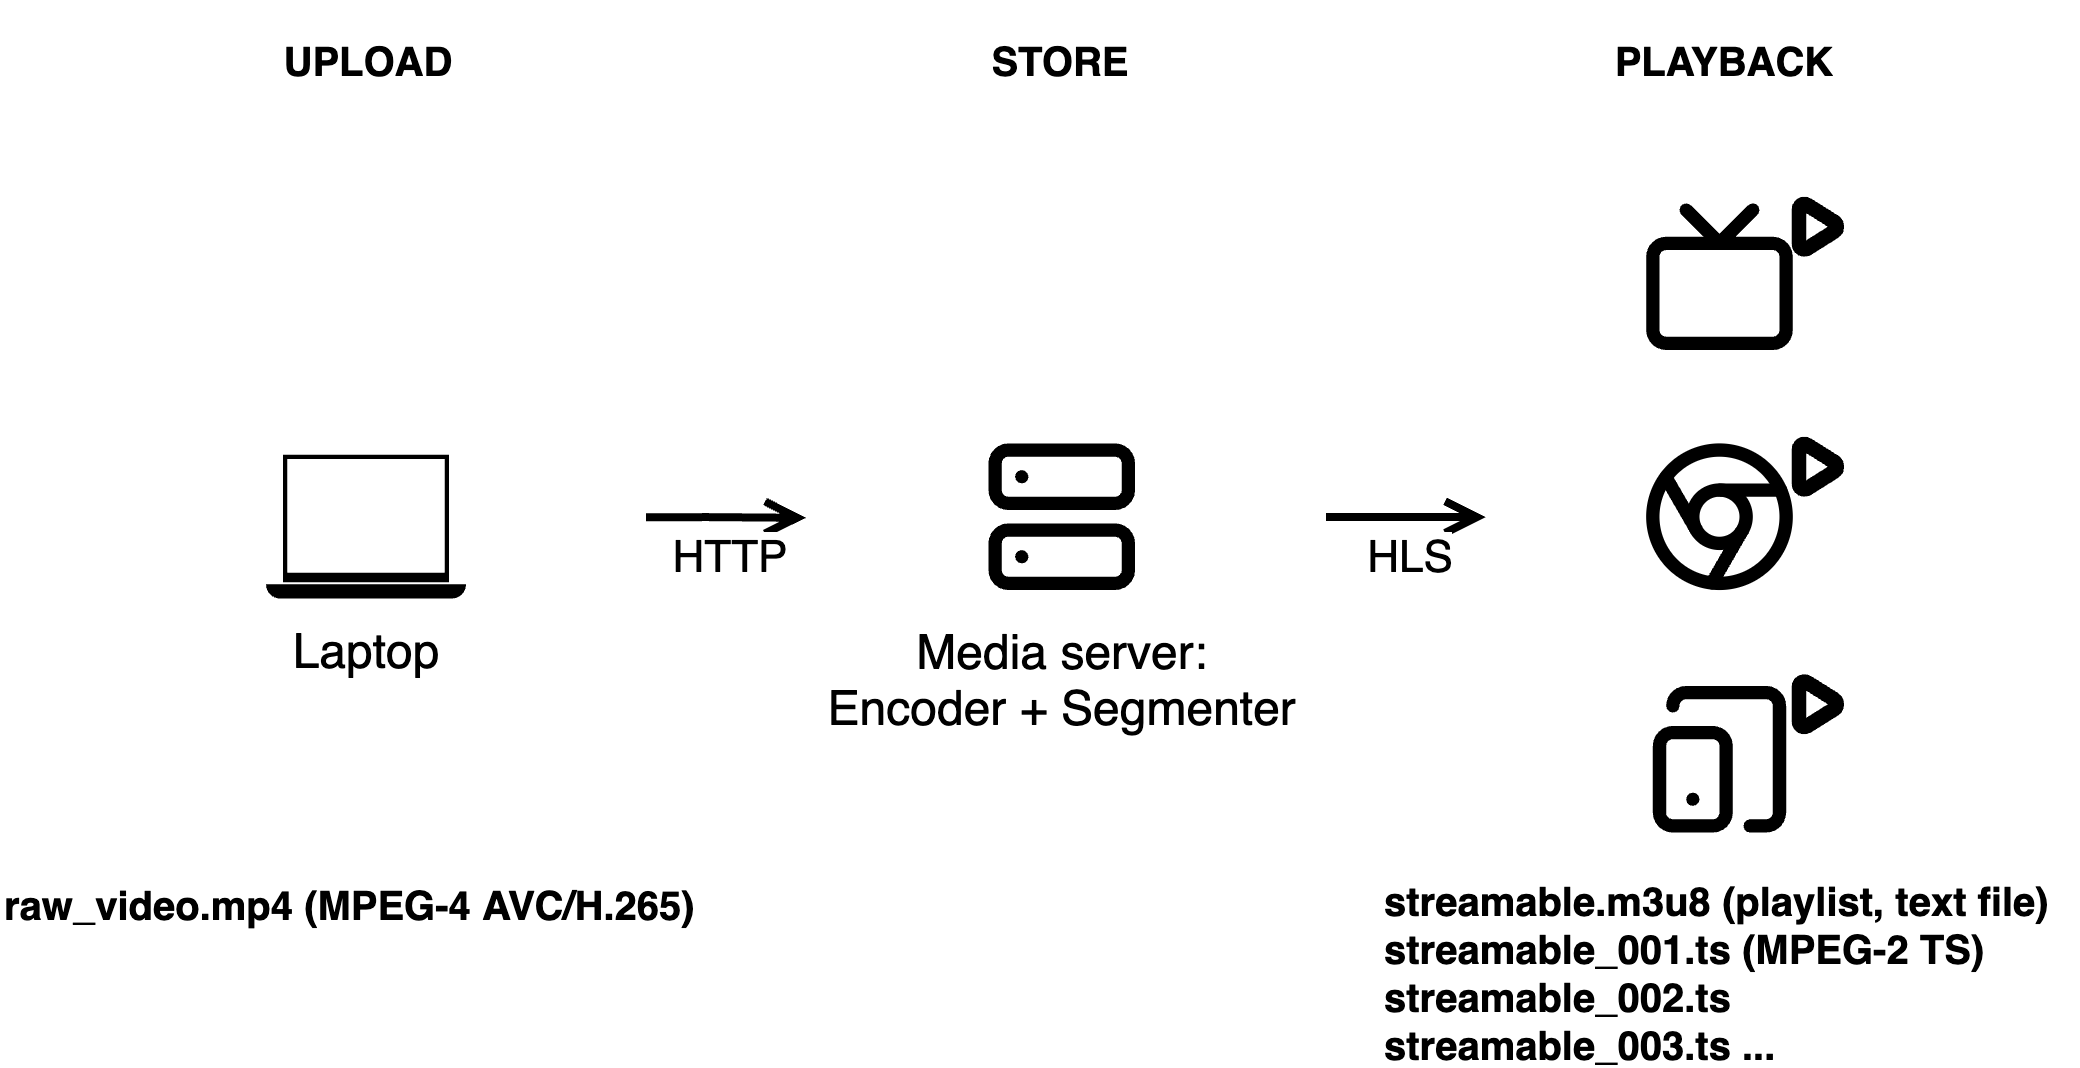
\includegraphics[width=120mm, keepaspectratio]{figures/dipterv_vodsetup.png}
	\caption{Példa egy VOD-kiszolgálás résztvevő eszközeire.}
	\label{fig:vodsetup}
\end{figure}

\begin{figure}
	\centering
	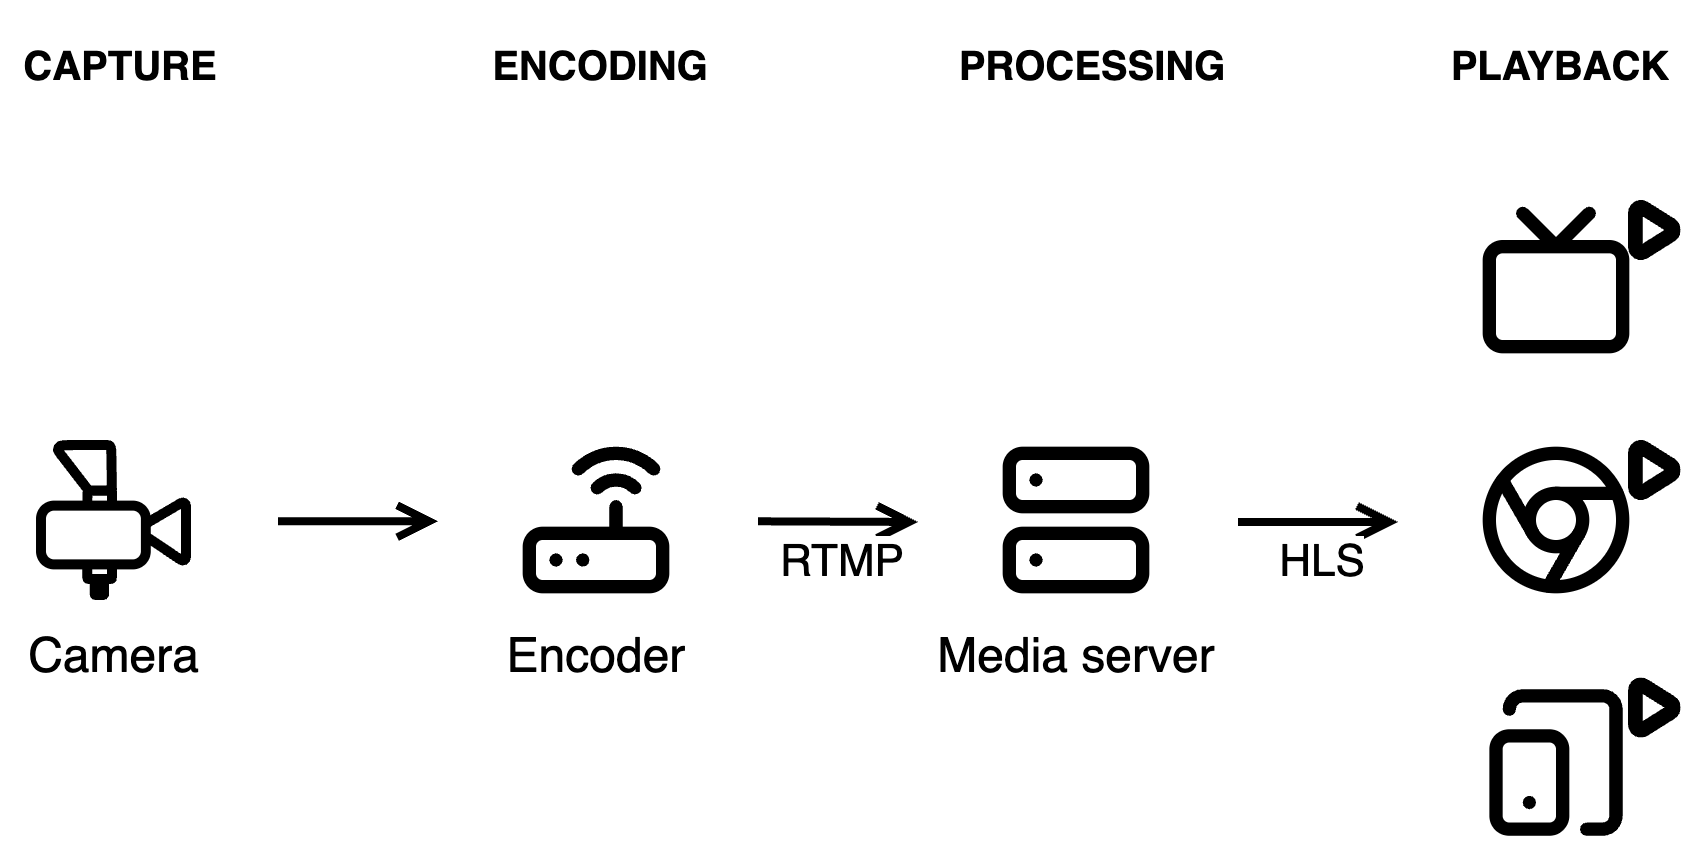
\includegraphics[width=100mm, keepaspectratio]{figures/dipterv_livesetup.png}
	\caption{Példa egy élő közvetítés résztvevő eszközeire.}
	\label{fig:livesetup}
\end{figure}

\subsection{Adaptive Bitrate Streaming}

A streamelést erősen befolyásoló tényező a hálózati feltételek változása, amelyek a videólejátszás minőségét és késleltetését is befolyásolják. Az Adaptive Bitrate Streaming (ABR) egy a hálózati kiszolgálás során alkalmazott technika, amely megoldást jelenthet erre a problémára.

Az ABR során a forrásvideót több különböző bitrátával dolgozó kodekekkel és különböző felbontással kódoljuk a médiaszerveren, majd lejátszáskor a lejátszó alkalmazás a hálózati feltételek változására reagálva, valamint a fogadó fél számítási kapacitásától függően valós időben választja ki a megfelelő vi\-de\-ó\-strea\-met ezek közül, onnan válogatja a packeteket (\refstruc{fig:ABR}).

\begin{figure}
	\centering
	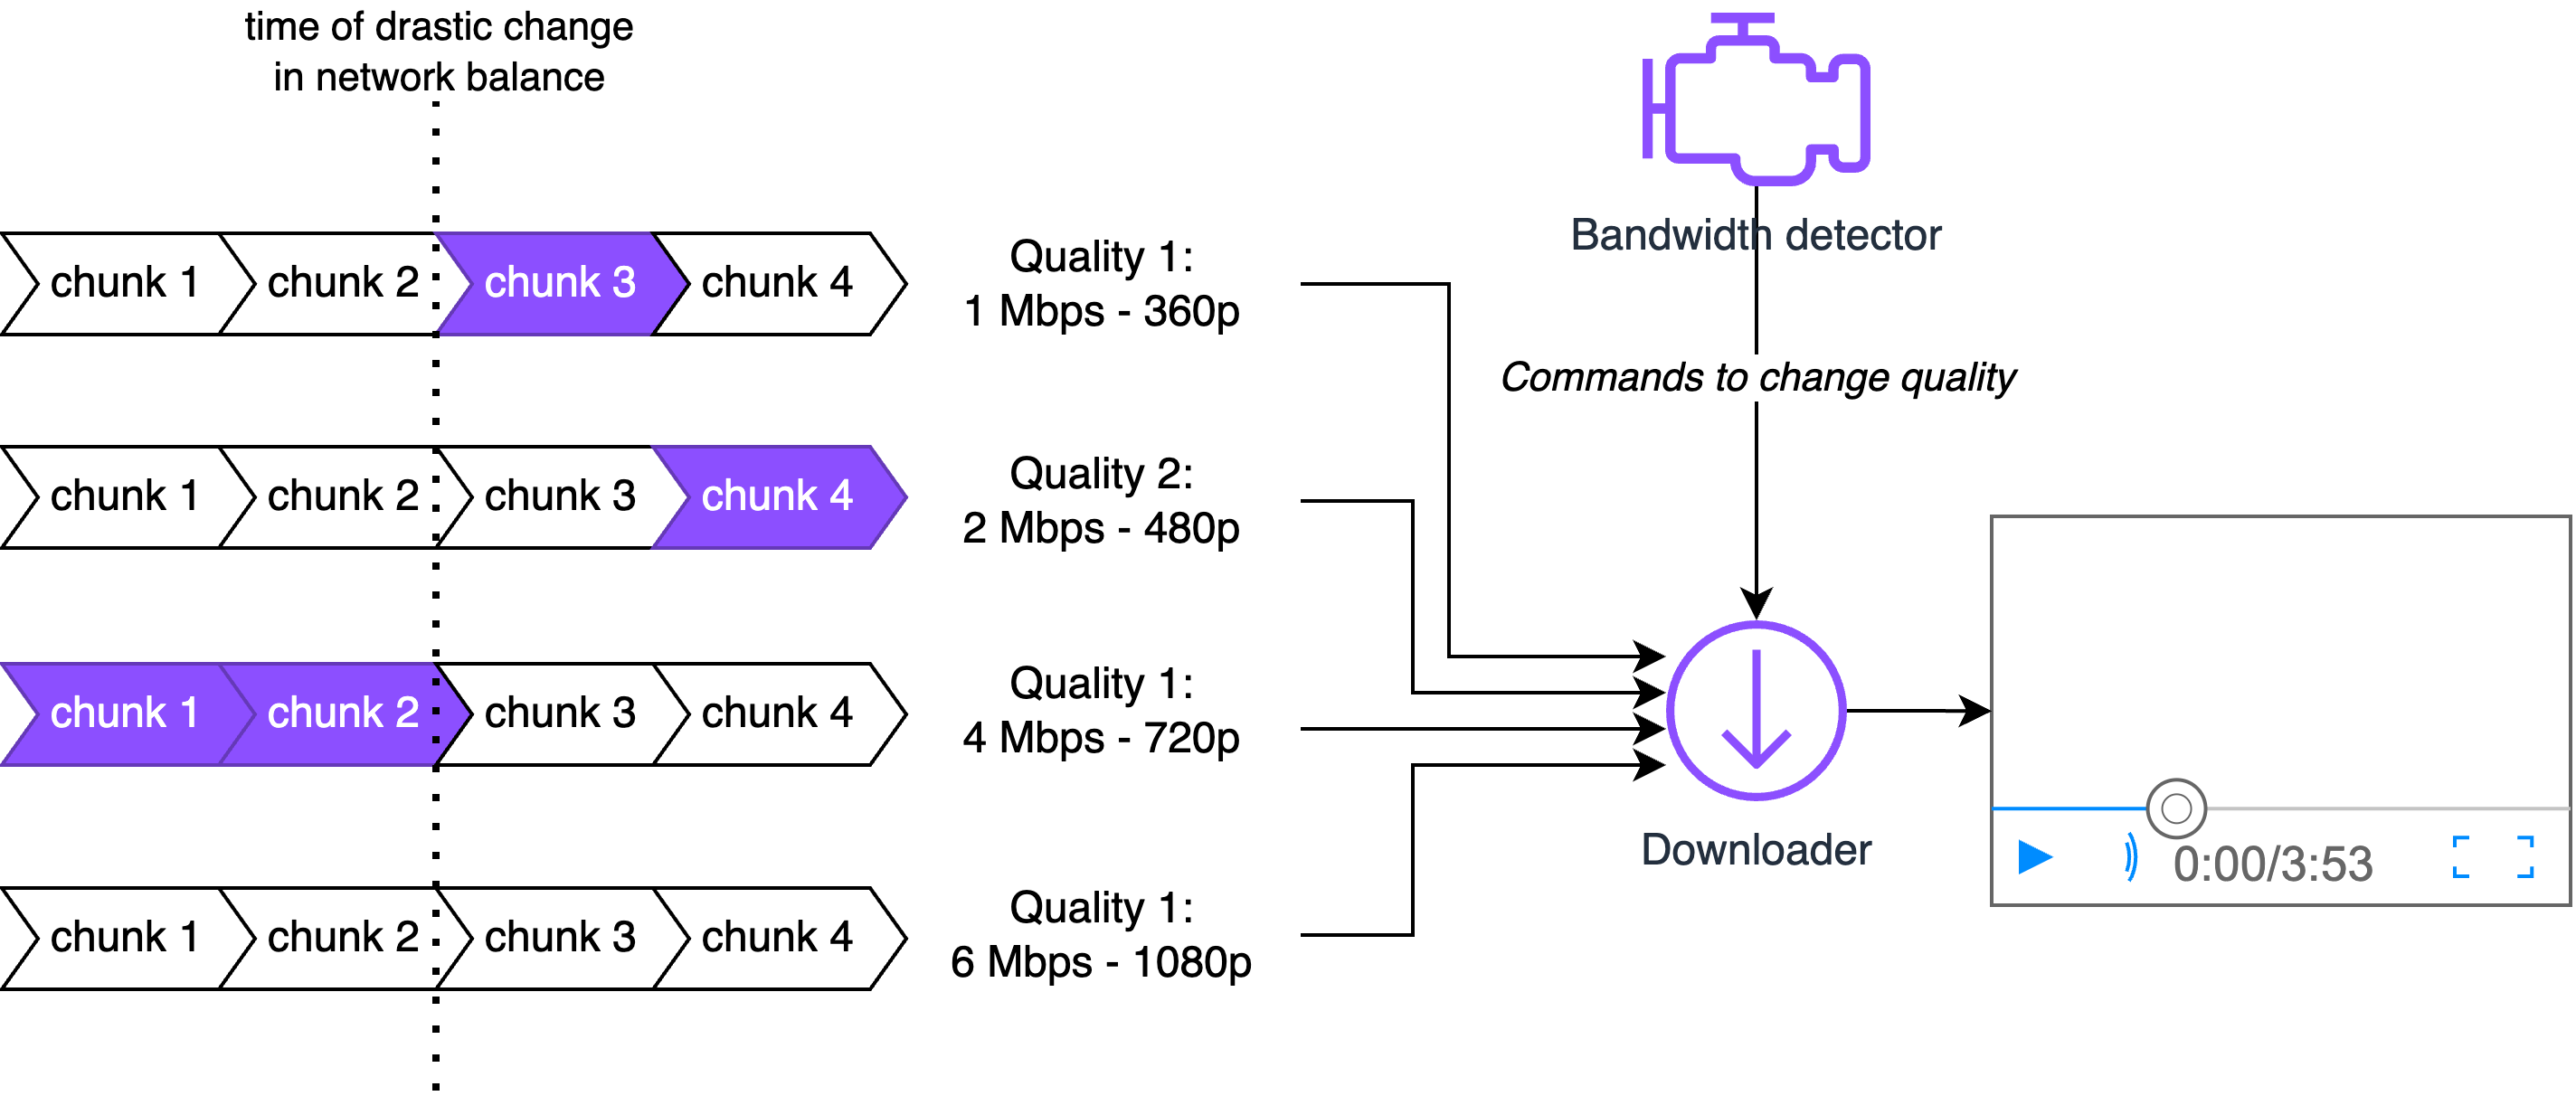
\includegraphics[width=140mm, keepaspectratio]{figures/dipterv_abr.png}
	\caption{Az Adaptive Bitrate Streaming működése.}
	\label{fig:ABR}
\end{figure}

Tiszta, hogy az ABR-t megvalósító rendszer előnyös mind a VOD, mind az élő közvetítés esetében, mivel a hálózati feltételek változása mindkét esetben előfordulhat, az automatikus streamváltogatás beavatkozás nélkül sokkal nagyobb Quality of Experience (röviden QoE, magyarul \emph{az élmény minősége}) lehetőségét tudja biztosítani \cite{DashAbr}. Az ABR-t alkalmazó rendszerek a videóadatokat több különböző bitrátával kódolják, ez természetesen a feldolgozási idejét a rendszereknek megnöveli, sőt élő közvetítés során egységnyi idő alatt jóval több számítási terhelést kell kibírnia a rendszernek.

\section{Videó streaming hálózati protokolljai}

Videó streamelésére -- másképp fogalmazva: valamely korábban ismertetett formátumban tárolt videófájl adatfolyamba való illesztésére -- különböző hálózati protokollok palettája áll rendelkezésünkre.

Néhány ismertebb streaming használatára kitalált protokoll létrejöttük időrendjében \cite{StreamingHistory}:

\begin{itemize}
	\setlength{\itemsep}{1pt}
  \setlength{\parskip}{0pt}
  \setlength{\parsep}{0pt}
	\item Real-Time Messaging Protocol (RTMP, 1996)
	\item Microsoft Smooth Streaming (MSS, 2008)
	\item Adobe's HTTP Dynamic Streaming (HDS, 2009)
	\item HTTP Live Streaming (HLS, 2009)
	\item WebRTC (2011)
	\item Dynamic Adaptive Streaming over HTTP (DASH, 2012)
\end{itemize}

Jelen alfejezet ezen alkalmazásrétegben alkalmazott protokollok (Layer 7) közül vizsgálja meg a legelterjedtebb protokollokat, megemlítve, milyen szállítási rétegű protokollokkal (Layer 4) tudnak együttműködni.

\subsection{Real-Time Messaging Protocol}

A Real-Time Messaging Protocolt (RTMP) nevű protokollt még a Macromedia nevű cég fejlesztette ki, amely vállalatot később az Adobe felvásárolta. Az RTMP egy teljes szervertől kliensig tartó protokoll, amely a Flash Player és a Flash Media Server közötti kommunikációra lett kifejlesztve eredendően. Közvetlen dolgozik a TCP felett, ennek nincs köze a HTTP-hez. \cite{StreamingHistory} Az RTMP-t még támogatja sok-sok platform, mert egész alacsony késleltetést lehet vele elérni, egészen alacsony ``költségű'', a Twitch és a YouTube is támogatja, hogy RTMP pull üzemmódjában tudjunk ezeken a platformokon élő adást fogadni, tehát szerveroldalon még használt, persze a Flash Player támogatásának 2020-as kivezetése miatt a protokoll használata kliensoldalon pedig visszaszorult.

\subsection{HTTP Live Streaming}

A HTTP-alapú streaming protokollok közül a legelterjedtebb a HTTP Live Streaming (HLS), amelyet az Apple fejlesztett ki 2009-ben. A HLS eredetileg az Apple jogvédett kereskedelmi protokolljaként indult, azóta viszont már szabad felhasználásúvá vált. Az Apple eszközök -- macOS, iOS -- alapértelmezetten támogatják ezt a protokollt, és a modern böngészők is támogatják a Media Source Extensions (MSE) API-n keresztül. Az HLS a HTTP felett dolgozik, egymástól függelten packetekre szedi a teljes kiszolgálandó videót, és az RTMP-hez képest ez így állapotmentes adatforgalmazást tud megvalósítani. \cite{StreamingHistory}

HLS használata során H.264 formátumban kell a videóadatokat kódolni, a hangot AAC, MP3 vagy Dolby szabványokkal lehet kódolni. A konténerformátumot tekintve is kötött, MPEG-2 Transport Stream (MPEG-TS) formátumot használhatjuk, vagy pedig az MP4-et -- fMP4 technikával, azaz \emph{fragmented MP4-gyel}, ehhez pedig a Common Media Application Format (CMAF) konténerformátumra kell átalakítani. \cite{Cmaf} A darabokra szedést követően a packeteket egy lejátszási listában (.m3u8 kiterjesztésű szöveges indexfájl) tartja számon a szerver, amelyet a lejátszó alkalmazások letöltenek, és a lejátszás során a megfelelő sorrendben és időzítéssel lejátszák. \cite{HlsApple} Lásd a példát egy 720p-s streamet leíró indexfájlra a \ref{lst:m3u8example}. kódrészletben.

A HLS egy olyan protokoll, amely magában hordozza az ABR implementációját is, kliensoldalon modern Media Source Extensions funkcionalitást támogató böngészőkben elterjedt használni a \emph{hls.js}\footnote{\url{https://github.com/video-dev/hls.js}} nevű JavaScript-könyvtárat, amely implementálja a HLS protokollt. A .m3u8 indexfájl definiálhat több másik ilyen indexfájlt is, amelyek a különböző bitrátájú videóstreameket képviselik (pl. egy \emph{1080p.m3u8} fájl és egy \emph{720p.m3u8} fájl írja le a playlistjét egy-egy bitrátájú streamnek).

\vspace{0.4cm}
\begin{lstlisting}[caption=Részlet egy .m3u8 indexfájlból.,label=lst:m3u8example,basicstyle=\small,]
#EXTM3U
#EXT-X-VERSION:3
#EXT-X-TARGETDURATION:4
#EXT-X-MEDIA-SEQUENCE:1
#EXTINF:4.000000,
skate_phantom_flex_4k_2112_720p1.ts
#EXTINF:4.000000,
skate_phantom_flex_4k_2112_720p2.ts
#EXTINF:4.000000,
skate_phantom_flex_4k_2112_720p3.ts
#EXTINF:4.000000,
skate_phantom_flex_4k_2112_720p4.ts
#EXTINF:4.000000,
skate_phantom_flex_4k_2112_720p5.ts
\end{lstlisting}

\subsection{Dynamic Adaptive Streaming over HTTP}

A Dynamic Adaptive Streaming over HTTP -- DASH vagy MPEG-DASH, tekintve a fejlesztője ennek is az MPEG csoport volt -- egy 2012-ben szabványosított protokoll. Hasonlít a HLS-hez, HTTP felett forgalmaz, sorozatba illeszt egymástól független packeteket. Ezeket a szegmentált packeteket egy manifestfájlban tartja számon a szerver (Media Presentation Description, MPD-fájl). \cite{Dash}

A HLS-hez képest ez a protokoll kodekagnosztikus, ami annyit jelent, hogy nem kötődik videókodekhez, használható H.264, H.265, akár VP9 is. \cite{DashIso} Igyekeztek ezzel a protokollal egyezményesíteni a tartalomvédelmet is, Common Encryptiont (CENC) használ titkosításra. Digitális jogkezelésre (Digital Rights Management, DRM) is agnosztikus. Amióta a HLS támogatja az CMAF konténerformátumban való szállítást, azóta könnyen át lehet arról állni akár DASH protokollra is, ugyanis a DASH is CMAF-alapú. A DASH a HTTP/2 protokollt is támogatja, sőt HTTP/3-at is már UDP felett.

A HLS-hez hasonló elvekkel dolgozik a DASH is, illetve ez is egy ABR technológiájú protokoll. A DASH implementációjára JavaScript motorral rendelkező kliensekben -- böngészők, mobiltelefonok stb. -- a \emph{dash.js}\footnote{\url{https://dashjs.org/}} könyvtárat használják legtöbb esetben.

\subsection{WebRTC}

A WebRTC (Web Real Time Communications) egy nyílt forráskódú projekt részeként alapult -- támogatják kódbázisának fenntartását mind a Google, a Mozilla és az Opera csapatai is --, egy protokoll böngészőalapú valós idejű kommunikáció kialakítására. Ezt használja a Discord, a Google Chat és egyéb webes videóchat-alkalmazások. \cite{StreamingHistory}

A források és a streamet figyelők számának kardinalitása szempontjából ez eltér az előzőekben ismertetettektől -- amelyek egy forrás és több befogadóra optimalizált --, ez viszont peer-to-peer (P2P) alapú, tehát oda-vissza jellegű streamlést kell biztosítson, emiatt a WebRTC a legjobb választás, amennyiben a felhasználási célja az, hogy a felhasználók közvetlenül egymással kommunikálhassanak, és nem szükséges közbeiktatni egy központi médiaszervert. Ezenkívül a WebRTC-t egyre szélesebb körben próbálják alkalmazni a videó streaming területén is one-to-many közvetítésre is. Szabad felhasználású kodekeket alkalmaz videó- és hangkódolás terén (pl.: Opus, VP9). \cite{WebRTC}

\chapter{Követelmények}

Egy nagyszabású, YouTube- vagy Netflix-szintű webes videóstreaming-szolgáltatás megvalósítása rendkívül összetett feladat, amely köré így kiterjedt technikai és üzleti követelményrendszert tudunk kialakítani. Egy ilyen rendszernek kezdetben biztosítania kell az alapvető funkciókat, amelyet hétköznapi webalkalmazások is megvalósítanak, mint például a videók lejátszása során felmerülő interakciók kezelése. Azonban ahogy a platformunk népszerűsége növekedhet, újabb és újabb infrastrukturális igények merülhetnek fel: ezek teszik ki a nem funkcionális követelményeket, amik kiterjednek például a tartalomterjesztés minőségére, a biztonsági felkészültségére a webalkalmazásnak.

A következőkben részletezem azokat a követelményeket, elvárásokat, amelyeket szem előtt tartottam a streaming szolgáltatás megtervezésekor és megvalósításakor.

\section{Funkcionális követelmények}

A streaming szolgáltatást alapvetően egy központosított kliensoldali webes felületen keresztül lehet elérni, azon keresztül tudják adminisztrátorok kezelni a tartalmat. Ennek a közvetlen frontoldali webes felületnek és a szolgáltatásainak a követelményeit érdemesnek tartottam csoportokba szedni:

\begin{itemize}
  \item Felhasználókezelésre vonatkozó funkciócsoport
        \begin{itemize}
          \item Habár a videók megtekintéséhez nincs szükség felhasználókezelésre és bejelentkezésre, viszont a videók kezeléséhez szükséges megvalósítani a felhasználók azonosítását és jogosultságkezelését.
          \item A felhasználók AuthSCH segítségével tudnak bejelentkezni a rendszer ``stúdió'' nevezetű aloldalára, ahol a rendszer azonosítja őket AuthSCH-s profiljuk alapján, automatikusan jön létre felhasználói fiókjuk, regisztrációra külön nincs szükség.
          \item A felhasználók közötti különbséget a rendszerben adminisztrátorok és normál felhasználók között teszem meg, az előbbieknek jogosultságuk van a videók feltöltésére és kezelésére, az utóbbiaknak csupán bejelentkezésre későbbi adminisztrátorrá válásra, amennyiben másik adminisztrátor úgy dönt.
        \end{itemize}

  \item Videóprojektek kezelésére vonatkozó funkciócsoport
        \begin{itemize}
          \item Az adminisztrátorok a ``stúdió'' aloldalon tudnak új videóprojekteket létrehozni, amelyekhez a rendszer automatikusan generál egy egyedi azonosítót, amelyet a videóprojekt URL-jében is használ.
          \item Egy videóprojekt létrehozása után tudunk a videókhoz tartozó metaadatokat adni, azokon módosítani, mint például a cím, leírás, borítókép, kategória, résztvevő stábtagok.
          \item A videóprojektben lehetőség van egy darab MP4 konténerformátumú videó feltöltésére.
          \item Van lehetőség a videóprojekt teljes törlésére.
          \item A feltöltés után a felhasználói felület visszajelzést kell adjon arról, hol tart a videó feltöltési folyamata, illetve a videókonvertálás folyamata a hálózati adatfolyamra való felkészítéshez.
        \end{itemize}

  \item Élő közvetítés kezelésére vonatkozó funkciócsoport
        \begin{itemize}
          \item Az oldal kezdetlegesen csupán egy élő közvetítés adását támogatja, az adminisztrátor a ``stúdió'' aloldalon tudja ezt az egyetlen élő közvetítést indítani.
          \item A rendszer biztosítja, hogy fogadja egy külső forrásból (pl.: OBS Studio alkalmazásból) a felstreamelt videót a felhőn át és azt továbbítja a nézőknek.
          \item Az oldalon kell, legyen egy útvonal a nézők számára, ahol a közvetítés élőben megtekinthető.
        \end{itemize}
\end{itemize}

\section{Nem funkcionális követelmények}

A rendszerrel szemben támasztott nem funkcionális követelmények megállapításakor igyekeztem olyan dolgokra a hangsúlyt tenni, amelyek inkább számomra jelentenek kihívást, mivel nem terveztem a webalkalmazást úgy elkészíteni, hogy az valódi használatra készüljön -- azaz valódi haszna legyen és legyenek élő felhasználói a nagyvilágból, csupán a kísérletnek volt része. Ezeket az elvárásokat a következőkben állapítottam meg:

\begin{itemize}
  \item Biztonság
  \begin{itemize}
    \item A megoldás kihasználja az AWS-felhő adta biztonsági lehetőségeket mind a hálózati struktúra kialakításakor, a webalkalmazás védelmezésére és a biztonságos kommunikáció (pl. HTTPS) kialakítására.
    \item A webalkalmazásban a felhasználók autentikációját és autorizációját a JWT tokenek segítségével oldom meg.
  \end{itemize}
  \item Hordozhatóság és könnyű karbantarthatóság
   \begin{itemize}
    \item Konténerizálom a szerveralkalmazást, hogy könnyen lehessen telepíteni és futtatni, egy egységként lehessen kezelni.
    \item A konténer és a buildelendő kódok automatikusan fordulnak és települnek a CI/CD-folyamat részeként.
    \item A frissítések könnyedén kezelhetőek, erre alkalmazásra kerül konténerképeket tároló Docker Registry is.
    \item Eseményvezérelt architektúra az alkalmazás egyes folyamatainak megvalósítására és a szerveralkalmazás köré, hogy könnyen kiterjeszthető lehessen új funkcionalitásokkal.
    \item Az infrastruktúra kód formájában (Infrastructure as Code, IaC) is dokumentált, hogy könnyen lehessen újraépíteni a rendszert.
  \end{itemize}
  \item Elaszticitás
  \begin{itemize}
    \item Alkalmazásra kerül olyan futtatókörnyezet, amelyben könnyedén lehet az erőforrásokat növelni és csökkenteni, hogy a rendszer mindig a szükséges kapacitással rendelkezzen.
    \item Alkalmazásra kerül a CDN használata, hogy a videók gyorsan és megbízhatóan érhetőek legyenek el a nézők számára.
  \end{itemize}
  \item Költséghatékonyság
  \begin{itemize}
    \item Olyan szolgáltatások használata, amelyek csak a valóban szükséges erőforrásokat használják fel, és csak akkor, amikor azokra szükség van.
    \item A szolgáltatásokat úgy tervezem meg, hogy a lehető legolcsóbban lehessen őket üzemeltetni a kísérletezés során.
  \end{itemize}
\end{itemize}

\chapter{Felhasznált technológiák}

A fejezet célja, hogy bemutassa a videó streaming szolgáltatások implementációjához felhasznált konkrét szoftvereket, webes és felhőszolgáltatásokat, és az azok közötti kapcsolatokat.

\section{FFMpeg szoftvercsomag}

Az FFMpeg\footnote{\url{https://www.ffmpeg.org/}} egy nyílt forráskódú és GPL-licenszelésű szoftvercsomag, amely képes videók és hangok kódolására, dekódolására, átalakítására (konvertálás), valamint streamelésre. \cite{ffmpeg} Az FFMpeg a legtöbb operációs rendszeren elérhető, és számos különböző formátumot, modern kodekeket támogat. Az FFMpeg a videók és hangok kódolására és dekódolására szolgáló kodekeket tartalmazza, valamint számos különböző formátumot támogat, beleértve az MPEG-4, H.264, H.265, VP8, VP9, AV1, AAC, AC-3, Opus, és sok más formátumot. Folyamatosan frissen tartják a kodekeket, aktív fejlesztőbázissal rendelkezik.

A lokális videókonvertálásra és streamelésre az FFMpeg-csomagból az azonos nevű ffmpeg parancssori interfészt használtam. Beépítettem a webszerver alkalmazásba egy külön szolgáltatásrészt, amely kihív a webszerver folyamatából és egy megfelelően felparaméterezett ffmpeg parancsot futtat a videókonvertálásra és streamelés megkezdésére aszinkron módon, a kimeneti fájlokat a megfelelő helyre menti.

A felhő alapú megoldásban már nem került felhasználásra az FFMpeg, mivel az AWS Elemental szolgáltatásokat használtam a videókódolásra és streamelésre, viszont a szoftvercsomag közvetlen megismerése a videókonvertálás folyamatának megértését és a konvertálási folyamatok felparaméterezési lehetőségeinek mélyebb átlátását segítette.

\section{Open Broadcaster Software}

Az Open Broadcaster Software Studio (OBS Studio\footnote{\url{https://obsproject.com/}}) egy nyílt forráskódú, szabad szoftver, amelyet elsősorban élő közvetítésekhez és képernyőrögzítéshez használnak. Elterjedt Twitch-felhasználók körében. A program támogatja a Windows, macOS és Linux operációs rendszereket, és számos beállítási lehetőséget biztosít a felhasználók számára. Az OBS lehetővé teszi több videó- és hangforrás kombinálását, ennek köszönhetően webkamera felvétele, mikrofon inputja, az éppen használt képernyő képe vagy előre rögzített videók is kombinálhatóak a stúdió műszerfalán.

A szoftver kompatibilis a legnépszerűbb streamingplatformokkal, így például a YouTube-ra és a Twitchre is lehet feltölteni vele, és lehetőséget biztosít saját egyedi RTMP-szerverekhez való csatlakozásra is annak felkonfigurálásával. Az OBS Studio megbízható eszköz azok számára is, akik professzionális szintű élő közvetítést szeretnének megvalósítani.

\section{Amazon Web Services}

Az Amazon Web Services (AWS) a világ egyik legjobban elterjedt, legnagyobb szerverfarmjait fenntartó, nagy hírű vállalatok által is megbízható felhőszolgáltatója. Felhasználói számára számítási, hálózati, adattárolási célokat megvalósító szolgáltatások széles palettáját kínálja. Felhasználják az AWS-t a mesterséges intelligencia területén; valamint kiterjedt adatbázisok, adatfeldolgozó rendszerek építésére; megbízható és könnyen skálázható webes szoftverrendszerek kialakítására.

A felhasználók a szolgáltatásokhoz az AWS Management Console webes felületen keresztül, vagy az AWS Command Line Interface (AWS CLI) parancssori interfészén keresztül férhetnek hozzá. Az egyes felhasználók fel tudnak állítani maguknak egy vagy több AWS-fiókot, amelyek a számlázás és a jogosultságkezelés szempontjából elkülönülhetnek egymástól.

A fiókon belül lehetőséget kapunk granuláris jogosultságkezelésre, azaz az egyes felhasználók, szolgáltatások, vagy szolgáltatásrészek számára különböző alacsony szintű jogosultságokat adhatunk meg.

Az AWS regionális adatközpontokat üzemeltet a világ számos pontján, amelyek közül a felhasználók választhatnak, hogy melyik adatközpontban szeretnének szolgáltatásokat futtatni.

A költségeket ``pay-as-you-go'' alapelv alapján számolják fel, azaz a felhasználók csak az általuk használt szolgáltatások számítási kapacitásáért, a tárhelyért, az adatközpontból kifelé történő hálózati forgalomért fizetnek.

\subsection{AWS Elemental}

Az Elemental Technologies 2006-ban indította vállalkozását streamingmegoldások eladására, egy fő mérföldkövük volt, amikor a szolgáltatásaikkal került közvetítésre a 2012-es nyári olimpiai játékok Londonban. Az Elemental Technologies 2015-ben került az Amazon Web Services tulajdonába, azóta az AWS Elemental néven futó szolgáltatásokat kínálja az AWS-felhőben. A fő célja a szolgáltatáscsomagnak, hogy óriási célközönségek számára is megbízható streamközvetítési megoldásokat kínáljon, amelyeket könnyen lehet skálázni, és amelyek a legújabb videókódolásokat és -technológiákat alkalmazzák. \cite{Elemental}

Szoftveres megoldásaik közé tartoznak a következők: 

\begin{itemize}
  \item \textbf{Elemental MediaConvert}: A MediaConvert egy felhőalapú videókódoló szolgáltatás, Software-as-a-Serviceként viselkedik, egy API-t ad, amelyen keresztül kódolási munkafolyamatokat (``jobokat'') indíthatunk. A MediaConvert támogatja a legnépszerűbb videóformátumokat, mint például a H.264, H.265, és a VP9, valamint a legújabb HDR (High Dynamic Range) és Dolby Vision technológiákat is. HLS streamre is képes felkészíteni a videókat. Csupán fel kell tölteni a forrásvideót egy S3 vödörbe, majd a konvertálás után a kimeneti videók számára is egy S3 vödröt tudunk megadni.
  \item \textbf{Elemental MediaLive}: Az Elemental MediaLive egy élő videókódoló szolgáltatás, amely lehetővé teszi a felhasználók számára, hogy élő videóadásokat fogadjanak és kódoljanak át a felhőben. A MediaLive támogatja a legnépszerűbb élővideó feltöltési protokollokat, így az RTMP-t is. Ennek a használata már bonyolultabb, mint a MediaConverté, nem szimplán csak egy API hívásaként kell elképzelni. Külön csatornákat lehet benne definiálni, azokhoz inputot/inputokat rendelni, ezután pedig a kódolási munkafolyamatokat felkonfigurálni. Az AWS sokféle nyelvben garantál SDK-kat, amelyek segítségével könnyen lehet automatizáltan MediaLive csatornákat indítani külön-külön adásokhoz.
  \item \textbf{Elemental MediaPackage}: Az Elemental MediaPackage készíti elő, csomagolja a videófolyamot hálózati protokollokon szállítmányozásra, garantálja a biztonságos és folyamatos tartalomtovábbítást. Biztosíthatja VOD-ok S3-ból való továbbosztását, vagy élők továbbosztását a MediaLive-ból. A MediaPackage támogatja a legnépszerűbb kliensfelőli protokollokat, mint például az HLS, DASH és a Microsoft Smooth Streaming. Könnyedén integrálható CloudFront disztribúciókba.
\end{itemize}

Érdemes még a szoftveres megoldások közt megemlíteni az Elemental MediaConnectet, amely egy Quality of Service (QoS) réteget biztosít a streamet fogadók és az AWS-felhő között, megbízható és biztonságos hálózati kapcsolatot biztosít. Ismert lehet még az Elemental MediaTailor, amely lehetővé teszi a reklámok beillesztését a videófolyamainkba. Korábban még a felhozatalba tartozott, azonban kivezetésre kerül már az Elemental MediaStore 2025. november 13-áig, amely egy objektumtároló szolgáltatás volt, viszont már az Amazon S3 kiváltotta, mivel az már erős read-after-write konzisztenciát tud biztosítani 2020 óta. \cite{Mediastore}

Ezeken kívül az AWS szolgáltat még fizikai hardvereket is a streaming könnyítésére és a nagy számításigények kiszolgálására, ezek közé tartozik például a AWS Elemental Link, amely egy HDMI- és SDI-portokkal rendelkező eszköz, lehetővé teszi a helyszíni videóforrások közvetlenül a felhőbe való továbbítását. A szoftveres és hardveres megoldások összekötésére egy példát szolgáltat mind VOD-ok és élőadások kiszolgálására a \refstruc{fig:vodlive}.

\begin{figure}[ht]
	\centering
	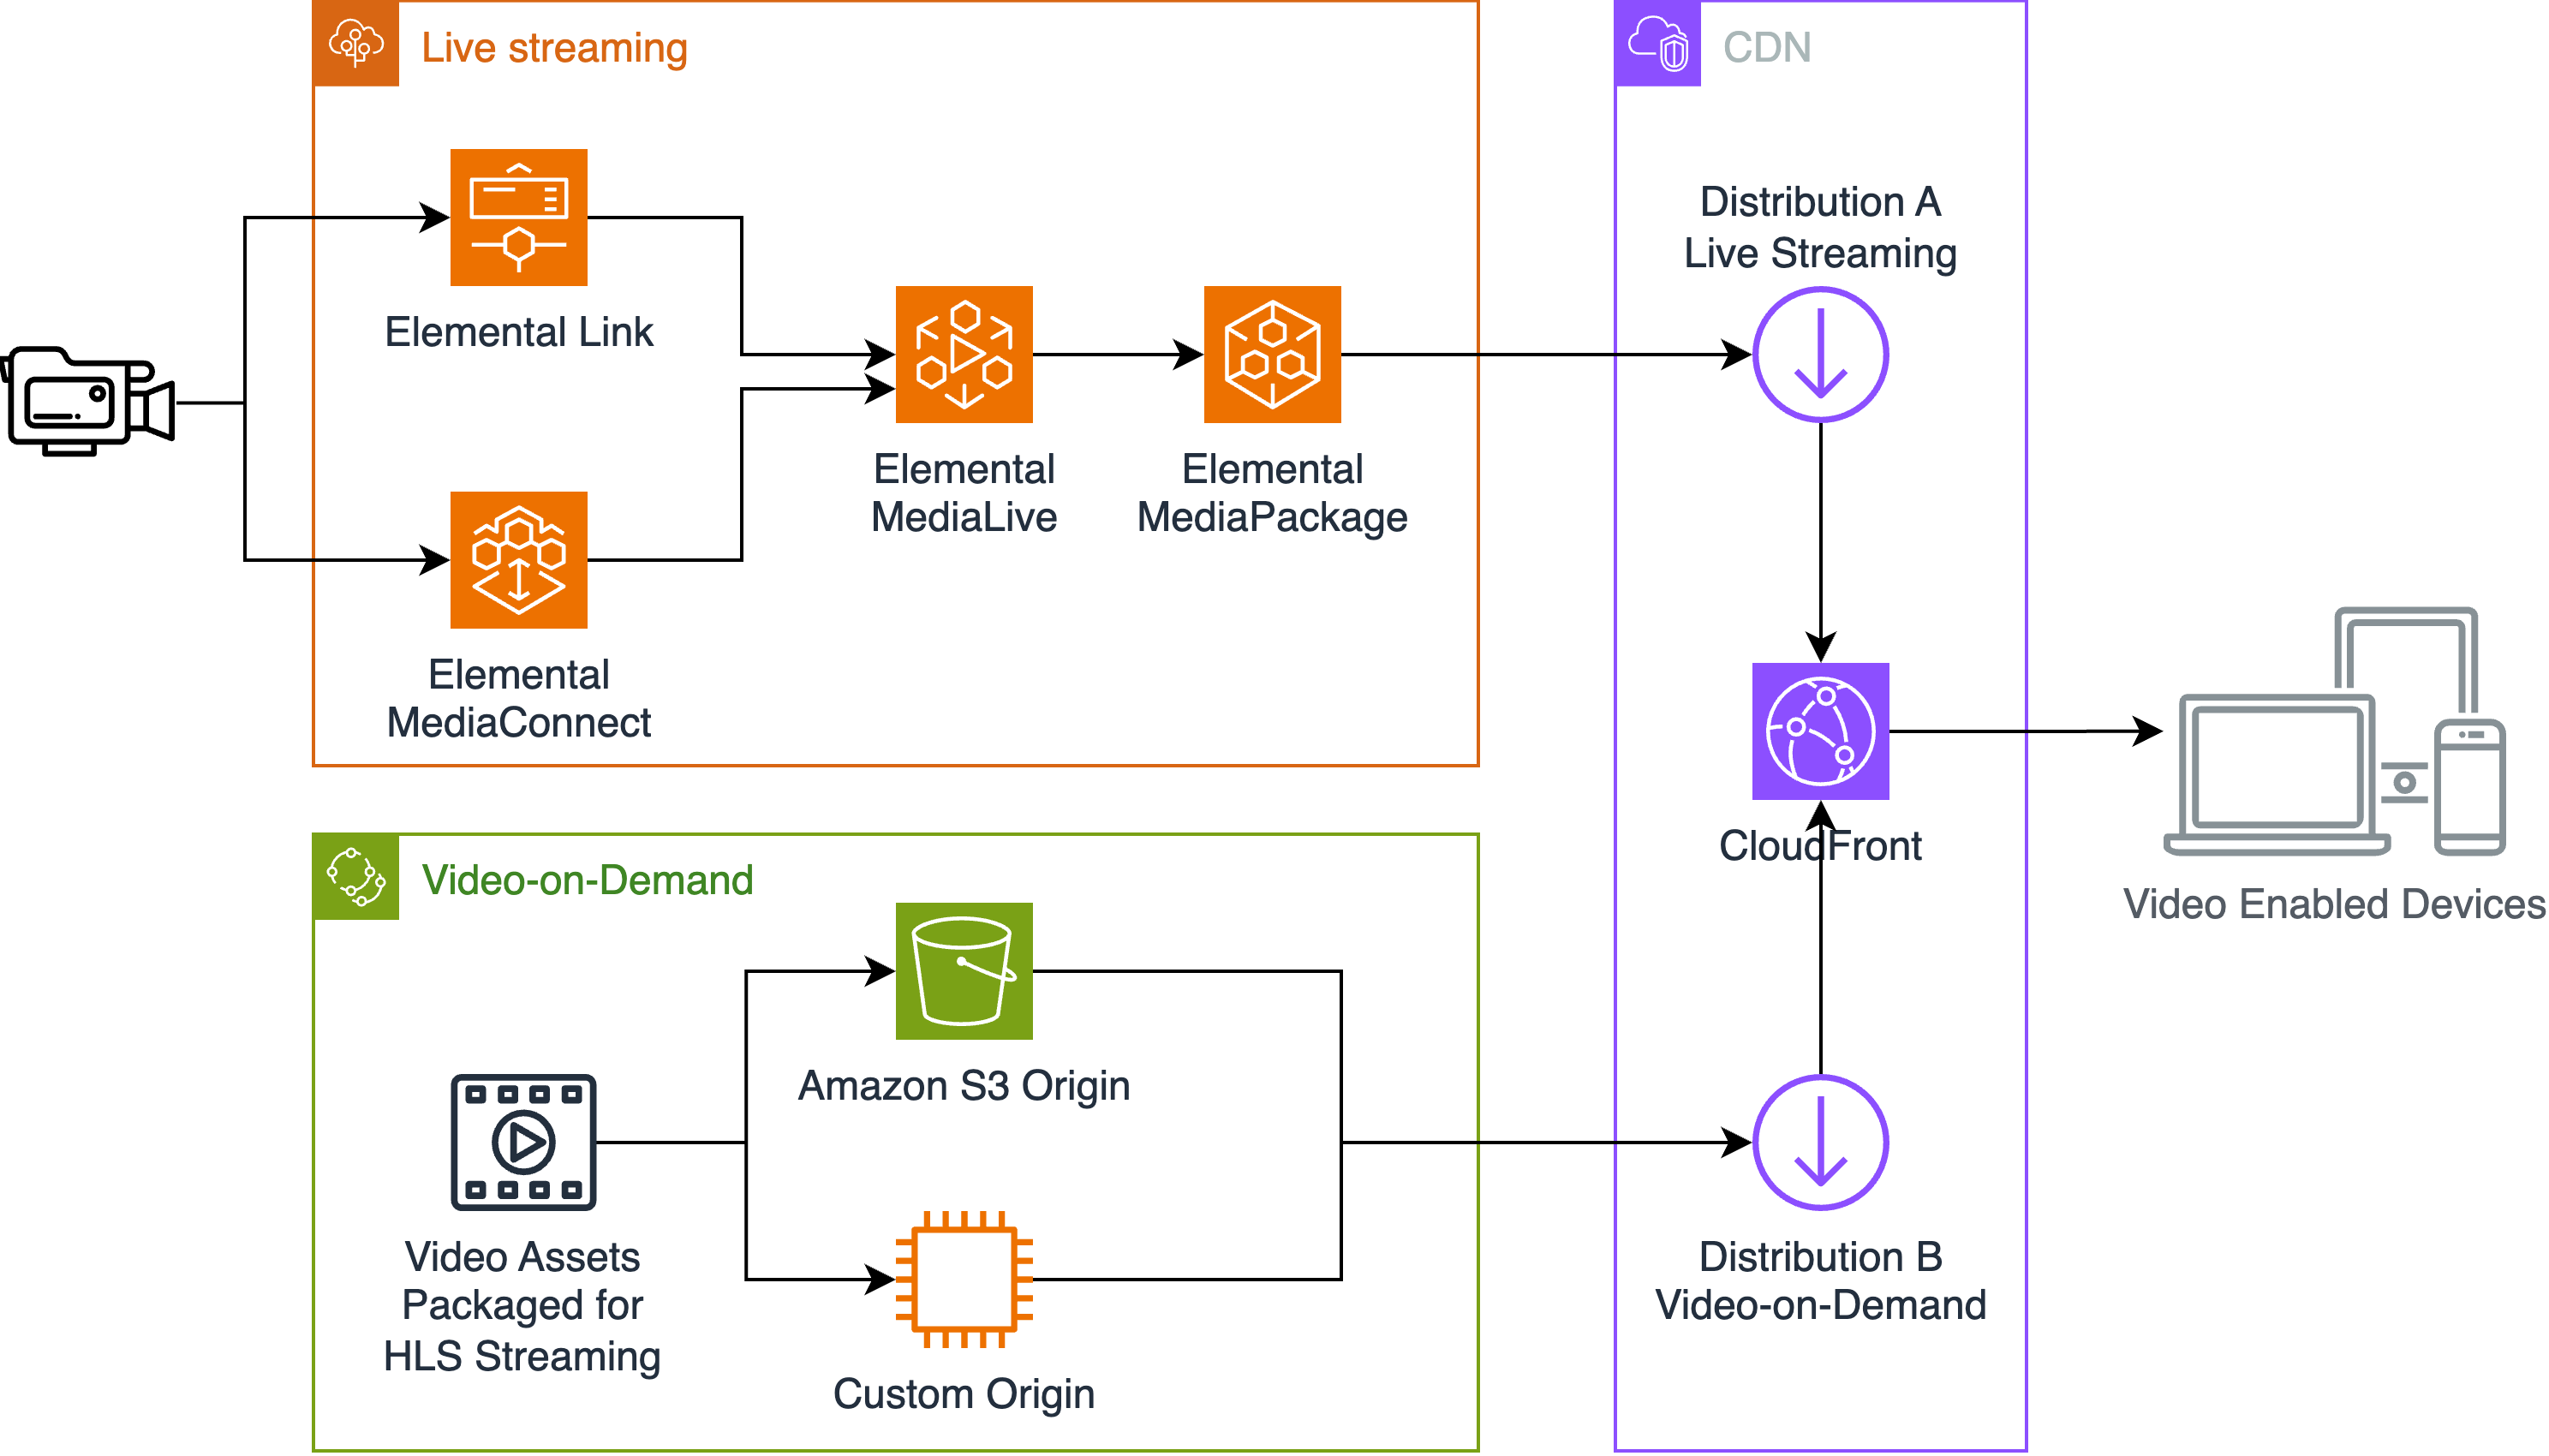
\includegraphics[width=120mm, keepaspectratio]{figures/dipterv_vodlive.png}
	\caption{Példa AWS Elemental szolgáltatások architektúrába kötésére.}
	\label{fig:vodlive}
\end{figure}

\subsection{Amazon IVS}

Az Amazon Interactive Video Service (IVS) egy teljesen AWS-kezelt, skálázható, és megbízható élő videó streaming Software-as-a-Service (SaaS), amely lehetővé teszi a fejlesztők számára, hogy gond nélkül integrálják az élő streaming funkcionalitását a saját alkalmazásaikba. Az IVS az Elemental szolgáltatásokhoz képest end-to-end megoldást kínál kis késleltetésű többnézős alkalmazásra: HLS-alapú kiszolgálás, körülbelül 5 másodperces késleltetést szokott biztosítani; valamint valós idejű alkalmazásra is: WebRTC-alapú kiszolgálás. \cite{Ivs} A forrásvideó-kódolástól a tartalomkiszolgálásig minden szükséges funkciót biztosít (\refstruc{fig:ivselemental}\footnote{A kép forrása: \url{https://aws.amazon.com/blogs/media/awse-choosing-aws-live-streaming-solution-for-use-case/}}), nekünk csupán a Software Development Kitjét (SDK) kell használni a saját alkalmazásunkban, és a többit az AWS-re bízhatjuk. Ezenkívül biztosít olyan funkcionalitásokat, mint chatszobák és szavazások szolgáltatása, amelyeket könnyen integrálhatunk ezekbe az adásokba.

\begin{figure}[ht]
	\centering
	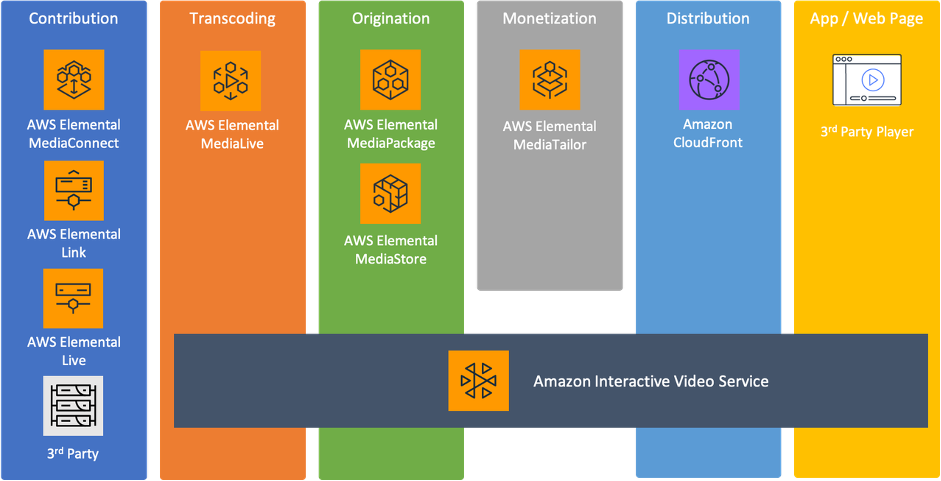
\includegraphics[width=120mm, keepaspectratio]{figures/aws_media.png}
	\caption{Amazon IVS és az AWS Elemental szolgáltatások összehasonlítása.}
	\label{fig:ivselemental}
\end{figure}

Ezen szolgáltatás ismertetése a megértést és a választás indoklását szolgálja későbbi fejezetekben, az Amazon IVS nem került felhasználásra a konkrét lefejlesztett rendszerben.

\subsection{Amazon VPC}

Az Amazon Virtual Private Cloud (Amazon VPC) egy virtuális hálózati környezet. Benne megvalósítható, hogy az AWS publikus felhőjén belül is privát és publikus saját hálózatokat hozzunk létre. Az Amazon VPC segítségével a felhasználók teljes kontrollt gyakorolhatnak a virtuális hálózati környezetük felett, beleértve a VPC-k alatti alhálózatok IP-tartományainak konfigurálását, útvonaltáblák kitöltését, a hálózati interfészek/portok korlátozásait, egyéb hálózati eszközök beillesztését (NAT Gateway-ek, Internet Gateway-ek, valamint Transit Gateway-ek), felülvizsgálható benne a hálózati teljesítmény.

\subsection{Amazon ALB}

Az Application Load Balancer (ALB) az Amazon Elastic Load Balancer (ELB) egy fajtája, ISO--OSI Layer 7 szinten, azaz alkalmazásrétegek szintjén működő terheléselosztó hálózati eszköz. Automatikusan skálázódik, lehetővé teszi a felhasználók számára, hogy egy vagy több szerver példány között egyenletesen eloszthassák a beérkező HTTP- és HTTPS-kéréseket. Az ALB képes a kéréseket a kérések fejlécei alapján vagy a kérések útvonala alapján elkülöníteni a forgalmat.

\subsection{Amazon S3}

Az Amazon Simple Storage Service (Amazon S3) egy objektumtároló szolgáltatás, amely lehetővé teszi a felhasználók számára, hogy nagy mennyiségű adatot tároljanak az AWS-felhőben ``vödrökben'' (bucketokban). Az objektum egy fájl és a fájlt leíró metaadatok közösen. A vödör az objektumok tárolója.

\subsection{Amazon CloudFront}

Az előző fejezet egy szekciójában már említetésre kerültek a CDN mint a video-on-demand alapú streaming szolgáltatások egyik kulcsfontosságú eleme. Az Amazon CloudFront egy globális CDN, amely lehetővé teszi a felhasználók számára, hogy a tartalmat hozzájuk közelebbi szervereken tárolt cache-ből töltsék le, ezáltal csökkentve a késleltetést, csökkentve a központi szerverek terhelését, és növelve a letöltési sebességet. Tartalmaink csoportosítására CloudFront ``disztribúciókat'' használunk.

A disztribúciók különböző URI-útvonalaikon akár különböző CDN-forrásokból -- úgynevezett ``originekből'' -- tudnak tartalmat kiszolgálni: ilyen origin lehet egy S3 vödör, AWS Elemental MediaPackage alapú élőadás-csatorna, Amazon Application Load Balancer (ALB) példány, vagy akár egy egyéni HTTP-szerver is saját doménnévvel.

\subsection{Amazon ECS}

Az Amazon Elastic Container Service (ECS) arra szolgál, hogy konténer alapú alkalmazásokat, szoftvercsomagokat futtathassunk a felhőszolgáltatónál. Az ECS segítségével a felhasználók könnyen futtathatnak és skálázhatnak konténereket anélkül, hogy a konténerek futtatásához szükséges infrastruktúra mélyén futó szervergépeket, valamint azok életciklusát, operációs rendszerének patchelését kellene kezelniük -- ezek menedzselését az AWS Fargate motor veszi át, mi csupán a környezeti paramétereket kell felkonfiguráljuk az igényeinknek megfelelően.

Ilyen paraméterek a konténerek képei, a konténerek alapvető számítási erőforrásai (CPU-magok száma, memória mérete), a konténerek hálózati beállításai (porttovábbítások, alkalmazott Security Group), a konténerek naplózása (hova továbbítódjanak a futtatás során a naplók), és a konténerek hozzáférési jogosultságai az AWS felhőn belüli más szolgáltatásokhoz. Könnyedén kapcsolható össze Amazon ALB példánnyal.

Tipikusan alkalmazott az ECS párban az Amazon Elastic Container Registry (ECR) szolgáltatással, amely egy konténerképek tárolására szolgáló privát Docker Registry, amely lehetővé teszi a felhasználók számára, hogy a konténerek képeit biztonságosan tárolják és kezeljék az AWS felhőben.

\subsection{Amazon RDS}

Az Amazon Relational Database Service (RDS) egy relációs adatbázis szolgáltatás, amely segít, hogy könnyen és hatékonyan hozhassunk létre, üzemeltessünk és skálázzunk relációs adatbázisokat az AWS-felhőben. Az RDS támogatja a legnépszerűbb relációs adatbázis motorokat, mint például a PostgreSQL, MySQL, MariaDB, Oracle, és SQL Server.

Képes automatikusan kezelni az adatbázisok frissítéseinek telepítését és a folyamatos biztonsági mentéseket. Mivel ezek is konkrét szervereket igényelnek, az RDS is könnyen integrálható az Amazon VPC hálózati környezetébe, a hálózati védelme is biztosítható.

\subsection{Kiegészítő AWS szolgáltatások}

A konténerek orkesztrációjának kiegészítésére számos könnyen élesíthető és ECS-hez integrálható szolgáltatás áll rendelkezésre az AWS-felhőben, amelyek közül a legelterjedtebbek az Amazon CloudWatch Logs, az AWS Lambda és a Amazon EventBridge.

Az Amazon CloudWatch Logs egy naplózó és monitorozó szolgáltatás, amely lehetővé teszi a felhasználók számára, hogy a konténerek futtatása során keletkező naplókat gyűjtsék, tárolják, és vizsgálják az ezekből származó metrikákat is akár.

Az AWS Lambda egy serverless Function-as-a-Service (FaaS) szolgáltatás, amely lehetővé teszi kód függvényszerű futtatását anélkül, hogy szükség lenne a szerverek vagy a futtatási környezet menedzselésére. A Lambda-függvény eseményekre reagálva kerül meghívásra, például HTTP kérésekre, adatbázis eseményekre, vagy más AWS-szolgáltatások eseményeire.

Ezzel kapcsolatban kerül a képbe az EventBridge, az AWS központi eseménykezelő szolgáltatása, amely lehetővé teszi az egyes AWS-felhőszolgátatásokon futó alrendszerek közötti kommunikációt. Segítségével szűrhetünk eseményekre, azokat könnyen továbbíthatjuk az egyes AWS-szolgáltatások között, a célpontja egy EventBridge által elkapott eseménynek ennek megfelelően egy Lambda-függvény is lehet.

\section{A webes komponensek technológiái}

A különböző felhőszolgáltatásokon futó kódbázisokat elterjedt webes technológiák segítségével fejlesztettem. Ezen technológiák kerülnek bemutatásra a következő szekciókban.

\subsection{TypeScript és JavaScript nyelvek}

A JavaScript egy dinamikusan és gyengén típusos, interpretált programozási nyelv, amelyet webes alkalmazások fejlesztésére használnak. A böngészőben is JavaScript fut legtöbbször modern keretrendszerek (React.js, Vue.js vagy Angular) támogatásával a Document Object Model (DOM) renderelésére, manipulálására, ezzel tudjuk lehetővé tenni a kliensoldali webes alkalmazások interaktív működését, a felhasználói események kezelését, a HTTP-kérések küldését.

Ezenkívül ez a nyelv használható szerveroldali környezetben is, az erre használatos Node.js egy futtatókörnyezet, amely lehetővé teszi a JavaScript kód futtatását a szerveroldalon is. A Node.js a V8 JavaScript motorra épül, amely a Google Chrome böngészőben is fut, eseményvezérelt architektúrában szolgál ki függvényhívásokat, és aszinkron I/O működést biztosít, ami lehetővé a blokkoló műveletek nélküli működést, maximalizálja a skálázhatóságot. \cite{Node}

A Node.js biztosítja különböző könyvtárakkal a HTTPS alapú hálózati kommunikációt, a fájlrendszer műveleteket, a processz kezelést, a környezeti változók olvasását. A funkcionalitások kiterjesztésére szokás használni JavaScript modulokat, ekkor kerül középpontba az Node Package Manager (NPM) ökoszisztémája. Az NPM csomagkezelő segítségével könnyen telepíthetünk többek között Model-View-Controller alapú (MVC) keretrendszereket is (Express.js, Nest.js), Object Relational Mapping (ORM) eszközöket (Prisma, TypeORM), SDK-kat (AWS SDK), vagy akár különböző adatbázis- és cache-kezelőkhöz drivereket (PostgreSQL, Redis) a webszerverünk kiegészítésére.

A TypeScript egy szuperhalmaza a JavaScriptnek -- azaz a JavaScript szintaxisát bővíti ki --, amely szigorú és statikus típusosságot ad hozzá. A nyelvben írt kód a TypeScript fordító segítségével JavaScript kóddá alakítható. A TypeScript segítségével a fejlesztők könnyebben tudják a kódjukat karbantartani, mivel a típusok segítenek a hibák felismerésében, statikus analízisben, és a kódolás során a fejlesztőknek segítségére lehet a kód kiegészítésében is. Mind kliens- és szerveroldalon is használatos, a Node.js natívan nem, de vannak futtatókörnyezetek, amelyek fordítás nélkül is már támogatja a TypeScript futtatását (pl.: Deno).

A TypeScript-alapú technológiákból felépülő ``stackek'' előnye, hogy a kliens- és szerveroldali kódokat ugyanabban a nyelvben írhatjuk meg, így a fejlesztőknek nem kell külön-külön nyelveket és környezeteket tanulniuk, és a kódok könnyebben átírhatók, újrahasznosíthatók, és könnyebben karbantarthatók.

Mellékesen érdemes még megemlíteni, hogy az AWS CloudFront szolgáltatása lehetőséget nyújt az felhasználóhoz közel futó edge szerverfarmokon nagyon kicsi számításigényű függvényeket futtatni, amelyeket a felhasználói kérésekre lehet közvetlen ráereszteni. Ezeknek két típusa is létezik, a CloudFront Functionök felprogramozása egy korlátozottabb nyelvi lehetőségekkel rendelkező JavaScriptben történik, míg a Lambda@Edge függvények logikája lehet Node.js futtatókörnyezet feletti JavaScriptben, illetve akár Python nyelven megírva.

\subsection{React}

A React\footnote{\url{https://react.dev/}} egy nyílt forráskódú JavaScript-könyvtár, amelyet a Facebook (ma Meta) fejlesztett ki még akkoriban belső fejlesztőeszközként. Single Page Applicationök (SPA) fejlesztésére használt. A React a komponensalapú fejlesztést támogatja, amivel úgy tudunk építkezni, hogy az felhasználói felületet (User Interface, UI) kisebb, újrahasznosítható építőelemekre bonthassuk. Az egyik fő előnye a virtuális DOM, amely hatékonyan kezeli a változásokat és javítja a teljesítményt.

A React alapvetően klienoldali renderelést (Client-Side Rendering, CSR) használ, ami azt jelenti, hogy az alkalmazás a böngészőben fut, és a szerver csak egy alapszintű HTML-t küld, hozzá a JavaScriptet. Azonban nagyobb alkalmazásoknál gyakran szükség van más renderelési módszerekre: Server-Side Rendering (SSR) esetén A React alkalmazás HTML-jét a szerver generálja le és küldi el a böngészőnek. Ez javítja a teljesítményt és a keresőoptimalizálást (Search Engine Optimization, SEO), mert a keresőmotorok számára az oldal már előre renderelve érkezik. Egy másik ilyen módszer a Static Site Generation (SSG), amely során az oldalak statikusan generálódnak a buildelési folyamat során. Ez gyors betöltési időt eredményez. A Next.js egy React köré épített keretrendszer, amely mind SSG- és SSR-funkcióval is rendelkezik.

Gyakori, hogy a keretrendszer nélkül csupán statikus weboldalakat generálunk React felhasználásával, a Vite egy olyan buildelési eszköz, amely gyorsítja a fejlesztési folyamatot, és képes React- -- és akár Vue.js- vagy egyéb -- könyvtárral írt TypeScript vagy JavaScript kódot is statikus weboldalakká generálni. A TypeScriptben írt React-kód fájlkiterjesztése .tsx, illetve .jsx, ha JavaScriptben írodik.

A React egy nagyon népszerű keretrendszer, amelyet a fejlesztők széles körben használnak, és amelynek számos kiegészítő könyvtára és eszköze van, amelyek segítségével gyorsan és hatékonyan lehet webes felületeket fejleszteni. Ennek megfelelően széleskörben támogatott és szeretett könyvtárakat lehet beépíteni a React-alapú alkalmazásokba, mint például a React Router, SPA-n belüli routingra; a TanStack Query, egyszerűsített állapotkezelő aszinkron kérésekre; a React Hook Forms, gyors és hatékony formkezelésre.

\section{Üzemeltetési technológiák}

Végül pedig a fejlesztés során használt üzemeltetési technológiákat ismertetem, amelyek segítik a karbantarthatóságot, amelyek segítségével a fejlesztők könnyen tudják a kódbázisból az alkalmazásokat futtatni, az infrastruktúrát felhúzni.

\subsection{Docker}

A virtualizáció egy típusa a konténerizáció, amely lehetővé teszi a fejlesztők számára, hogy az alkalmazásokat virtuális gépeknél egyszerűbb ``konténerekbe'' csomagolják, abból képet generáljanak, azt pedig könnyen osszák tovább, és ezekből a képekből konténereket futtathassanak a számítógépükön vagy épp a felhőben. Egy virtuális gép a gazda gép hardvereit virtualizálja, a konténer pedig a gazda operációs rendszert virtualizálja, azaz a konténerek alatt közös a kernel (\refstruc{fig:virtudocker}\footnote{A kép forrása: \url{https://www.atlassian.com/microservices/cloud-computing/containers-vs-vms}}). Ezzel elveszik a teljes izoláció, azaz a biztonság, de a konténerek könnyebbek, gyorsabban indulnak (nincs bootolási idő), és kevesebb erőforrást használnak. 

A konténer egyfajta szabványosított egység, amely tartalmazza az alkalmazás kódját, a szükséges függőségeket (könyvtárakat), a konfigurációs fájlokat, és amire az alkalmazásnak szüksége van a futtatáshoz.

\begin{figure}[ht]
	\centering
	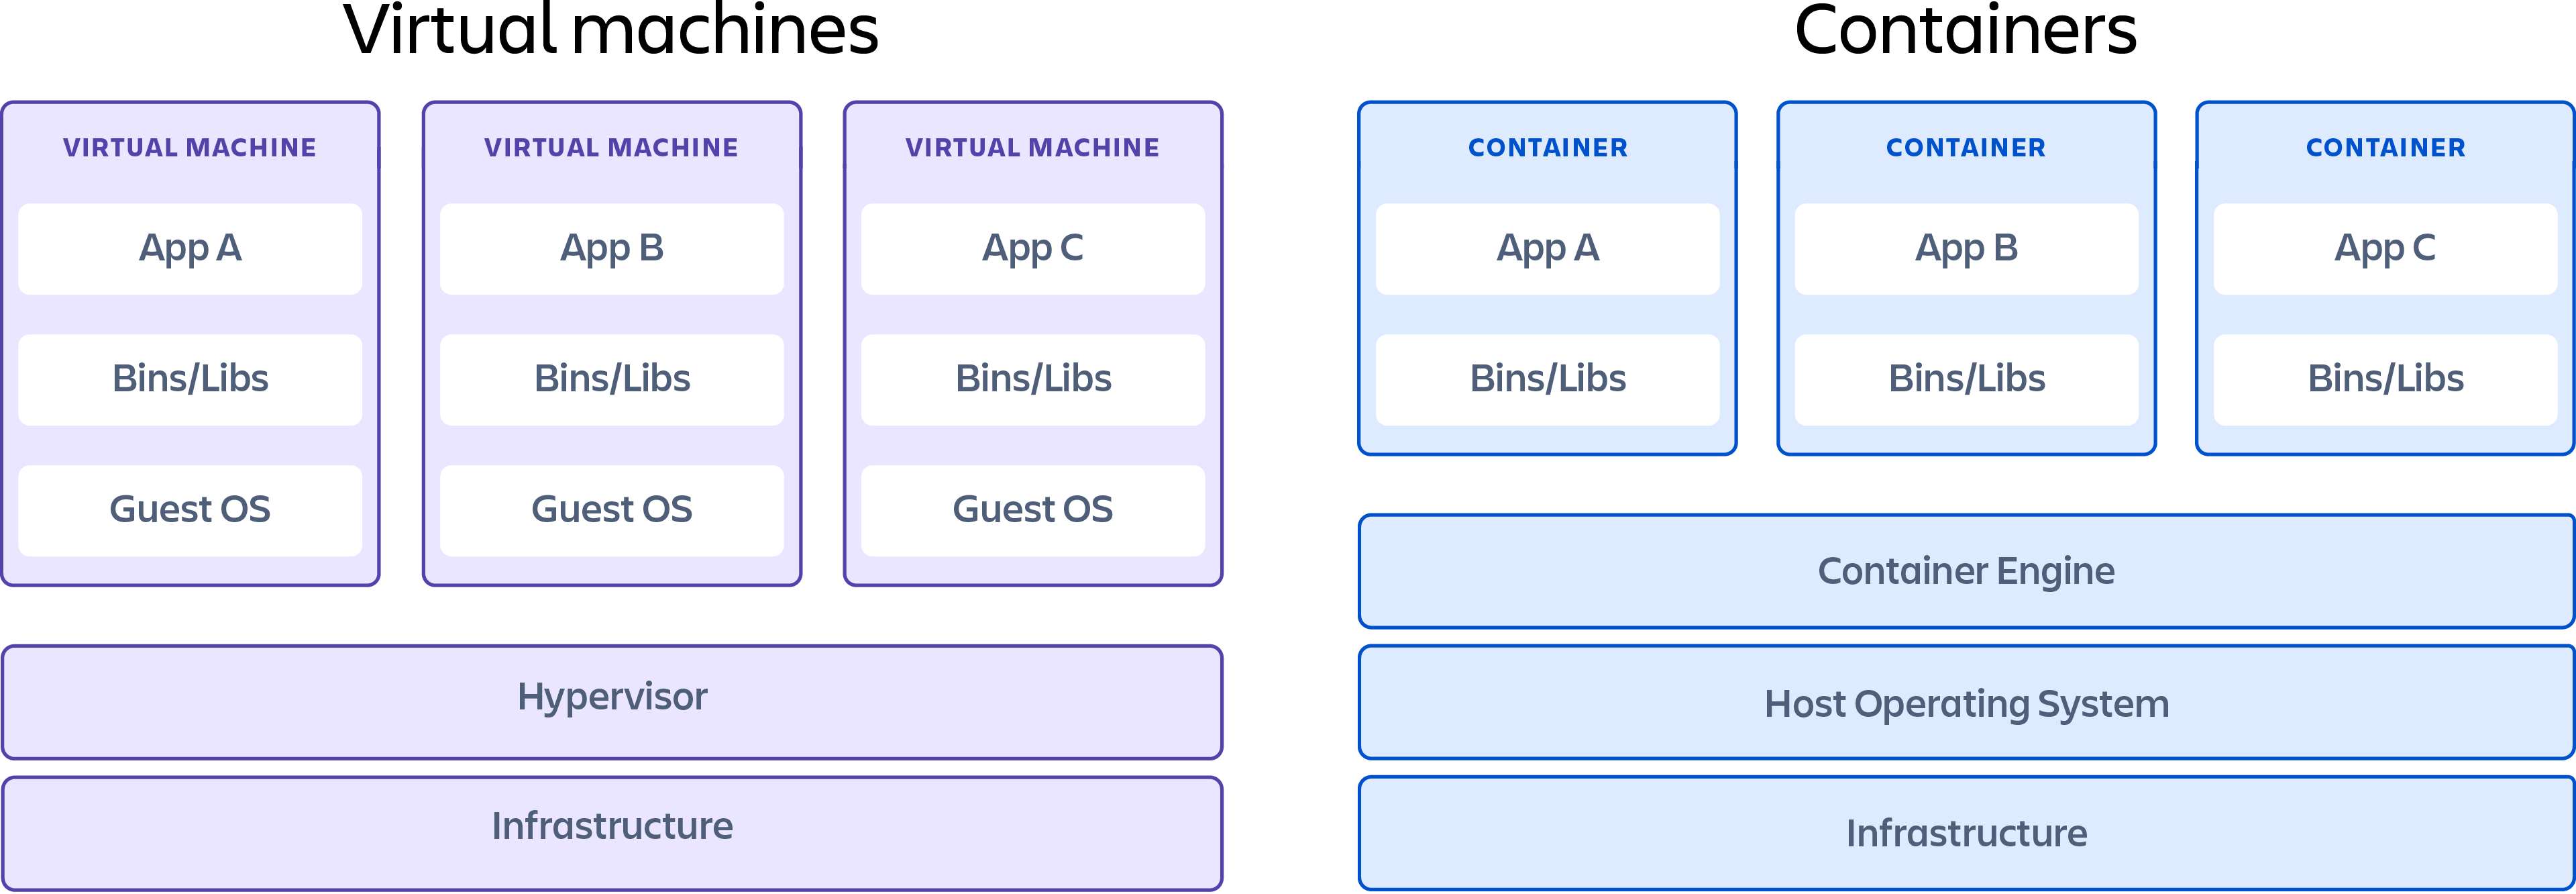
\includegraphics[width=120mm, keepaspectratio]{figures/virtudocker.png}
	\caption{Virtuális gépek és konténerek architekturális összehasonlítása.}
	\label{fig:virtudocker}
\end{figure}

A Docker egy konténerizációs fejlesztői környezet, a mélyén a containerd motor fut konténerizációs futtatókörnyezetként. \cite{Docker} Lehetővé teszi a konténerek létrehozását, indítását, kezelését és átvitelét. Virtuális tárhelyet és hálózatot biztosít a konténerek számára, és lehetővé teszi a konténerek közötti biztonságos kommunikációt. A Docker egy nyílt forráskódú projekt, amelyet a fejlesztők széles körben használnak a konténerizált alkalmazások fejlesztésére és futtatására.

\subsection{GitHub}

Szoftverrendszerek, alkalmazások fejlesztése során szinte elengedhetetlen a verziókezelés, amelynek segítségével a fejlesztők nyomonkövethetik a kódbázis változásait, visszaállíthatják az előző verziókat, és könnyen együtt tudnak dolgozni a kódon. Erre a munkafolyamatra az egyik legelterjedtebb Source Code Management (SCM) eszköz a Git verziókezelő. A Git egy elosztott verziókezelő rendszer. Minden fejlesztő saját gépén tárolja a teljes kódbázisát, majd a módosításokat a felhőben lévő tárolóval szinkronizálhatja.

A Git szoftver köré széleskörben találhatunk felhőtárhely-szolgáltatókat, ezek közül a legnépszerűbb a GitHub\footnote{\url{https://github.com/about}}. A GitHub a tárhelyen kívül sok más funkcionalitást is szolgáltat a hatékony együttműködés és kódgondozás kivitelezésére, egy ilyen szolgáltatása a GitHub Actions, amely CI/CD-folyamatok kezelésére egy eszköz, olyan folyamatokra hasznosítható, mint a statikus ellenőrzés, a building folyamatok automatizálása, és például a kód AWS-re való kiélesítése is.

\subsection{Terraform}

A Terraform\footnote{\url{https://www.terraform.io/}} egy elterjedt Infrastructure as Code eszköz, amely lehetővé teszi a felhasználók számára, hogy infrastruktúrát definiáljanak kódban, és ezt az infrastruktúrát automatizáltan hozzák létre, módosítsák és töröljék. A Terraform a felhőszolgáltatók API-jait, CDK-jait (Cloud Development Kit) használja az változtatások érvényre juttatására. Go nyelven íródott a motorja, a Terraform IaC-ra pedig a saját HCL (HashiCorp Configuration Language) nyelvét ajánlja, amely egy deklaratív nyelv.

\chapter{A tervezett architektúra}

TODO: Gyors bevezető arról, hogy külön AWS accountba dolgoztam és felügyeltem a költségeim.

\section{Logikai felépítés}

TODO: High-level leírása az AWS accounton belüli/datacenteren belüli hálózati kommunikáció rétegeinek.

\subsection{Összehasonlítás egy hasonló rendszerrel}

A tervek igazolásához segítségül kerestem az interneten nyílt forráskódú hasonló megoldásokat is. Megtaláltam a Technische Universität München (TUM) egy hallgatói csoportja, a TUM-Dev által fejlesztett az egyetemen is használt VoD és live streaming szolgáltatását, a GoCastot\footnote{\url{https://github.com/TUM-Dev/gocast}}. Ez a rendszer önállóan hosztolható szoftvereket komponál össze, nem felhőnatív. A rendszerben hasonló absztrakt terveket lehet megfigyelni az én megoldásaimhoz (\refstruc{fig:gocast}), ugyanígy HLS-sel szolgálják ki a tartalmakat (lásd \emph{TUM-Live Edge} példányok), viszont a live streamingre saját több portos workereket alkalmaznak (lásd \emph{TUM-Live-Worker} példányok), lehetőség ad viszont saját streamerből RTMP-n keresztül feltölteni élő közvetítést, ahogy én is megvalósítom a saját megoldásomban. Külön mikroszolgáltatás biztosítja a live és VOD streamingen kívüli funkcionalitásokat, a TUM-Live. Ez a megoldás nem teszi lehetővé, hogy a rendszeren kívül készült videót lehessen feltölteni és VOD-ként elérhetővé tenni rajta keresztül.

\begin{figure}[ht]
	\centering
	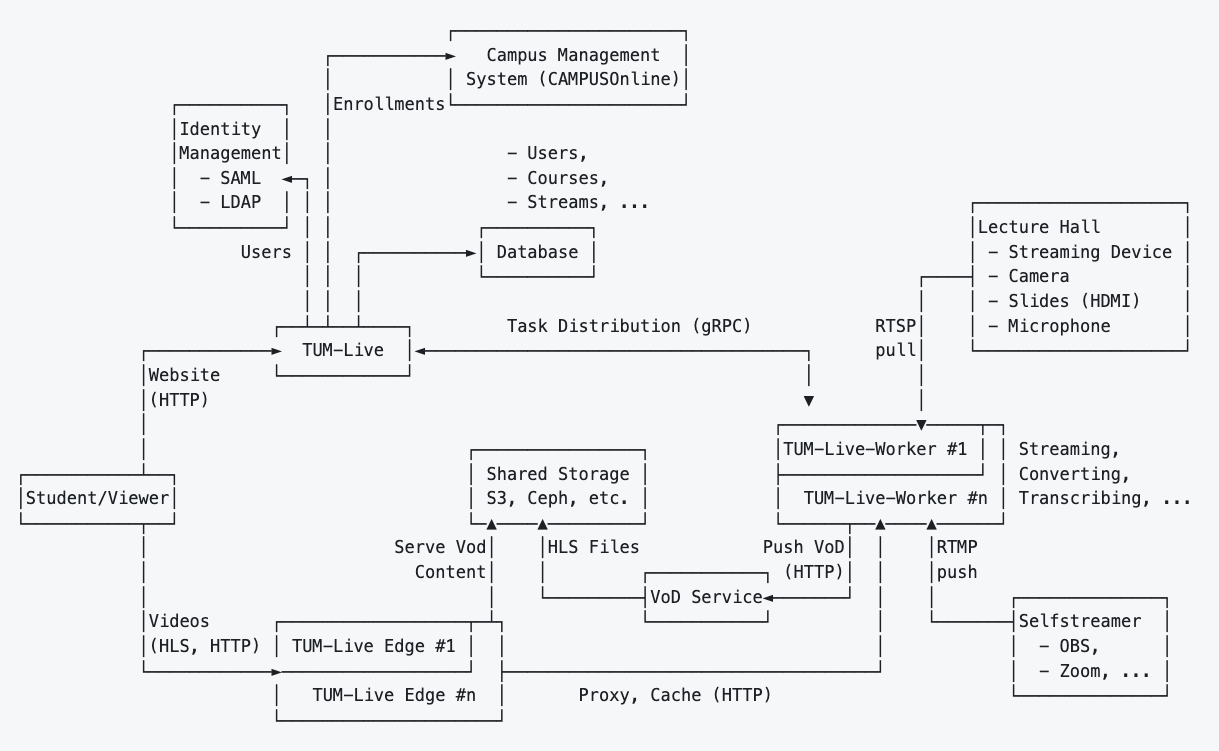
\includegraphics[width=140mm, keepaspectratio]{figures/gocast.png}
	\caption{A GoCast architektúrája a dokumentációból.}
	\label{fig:gocast}
\end{figure}

\section{Video-on-Demand kiszolgálás folyamata}

TODO: High-level leírása a VoD kiszolgálás folyamatának, megemlítve, melyik választott szolgáltatások vesznek részt ebben.

\section{Live streaming folyamata}

TODO: High-level leírása a live streaming folyamatának, megemlítve, melyik választott szolgáltatások vesznek részt ebben.

\section{Konfigurációmenedzsment}

TODO: Terraform választásának indoklása. Kialakított Terragrunt module rendszer. GitHub actions a Terraform tervek előnézetére, OIDC felállítása az AWS role felvételére.

\chapter{Kliensközeli komponensek implementációja}

A következőkben részletezem a klienseket kiszolgáló infrastrukturális komponensek konfigurációját, valamint a legfelső megjelenítési réteg szoftveres komponenseinek implementációját. A forgalom először a CDN-nel ütközik, amelyen keresztül lesznek elérhetőek a statikus weboldal erőforrásai, valamint a média-erőforrások csatornái.

\section{A CDN és a hozzácsatolt erőforrások}

A CDN és az ahhoz tartozó erőforrások jelentik az első belépési pontját egy a rendszerhez intézett kérésnek. A rendszer és a CDN -- azaz a Cloudfront disztribúció -- számára a \verb|stream.trisz.hu| doménnevet rendeltem, amelyet a saját \verb|trisz.hu| doménem aldoménjeként jegyeztem be a Route 53 szolgáltatásban egy külön DNS zónaként. A böngészőből, azaz kívülről indított kérések minden esetben a DNS feloldásával kezdődnek, a Route 53 névszervereire oldódik fel, ezzel szerzi meg a kliens az IP-jét a Cloudfront edge szerverfarmjának. A Cloudfront disztribúcióknak különleges CNAME rekordjaik vannak, biztosítják hogy a kliens a legközelebbi edge szerver farmhoz csatlakozhasson, a konkrét működést az AWS elrejti a háztető alatt előlünk. A biztonságos, HTTPS-alapú szerver-kliens kommunikációt a Cloudfront disztribúcióhoz tartozó SSL-tanúsítvánnyal biztosítja a rendszer. A tanúsítványt az AWS Certificate Manager szolgáltatásban generáltam és kezeltem, amely automatikusan megújítja a lejáró tanúsítványokat (\refstruc{fig:distro}), amennyiben a domainhez tartozó DNS zónát a Route 53 szolgáltatásban -- azaz az AWS szolgáltatásában kezeljük.

\begin{figure}[ht]
  \centering
  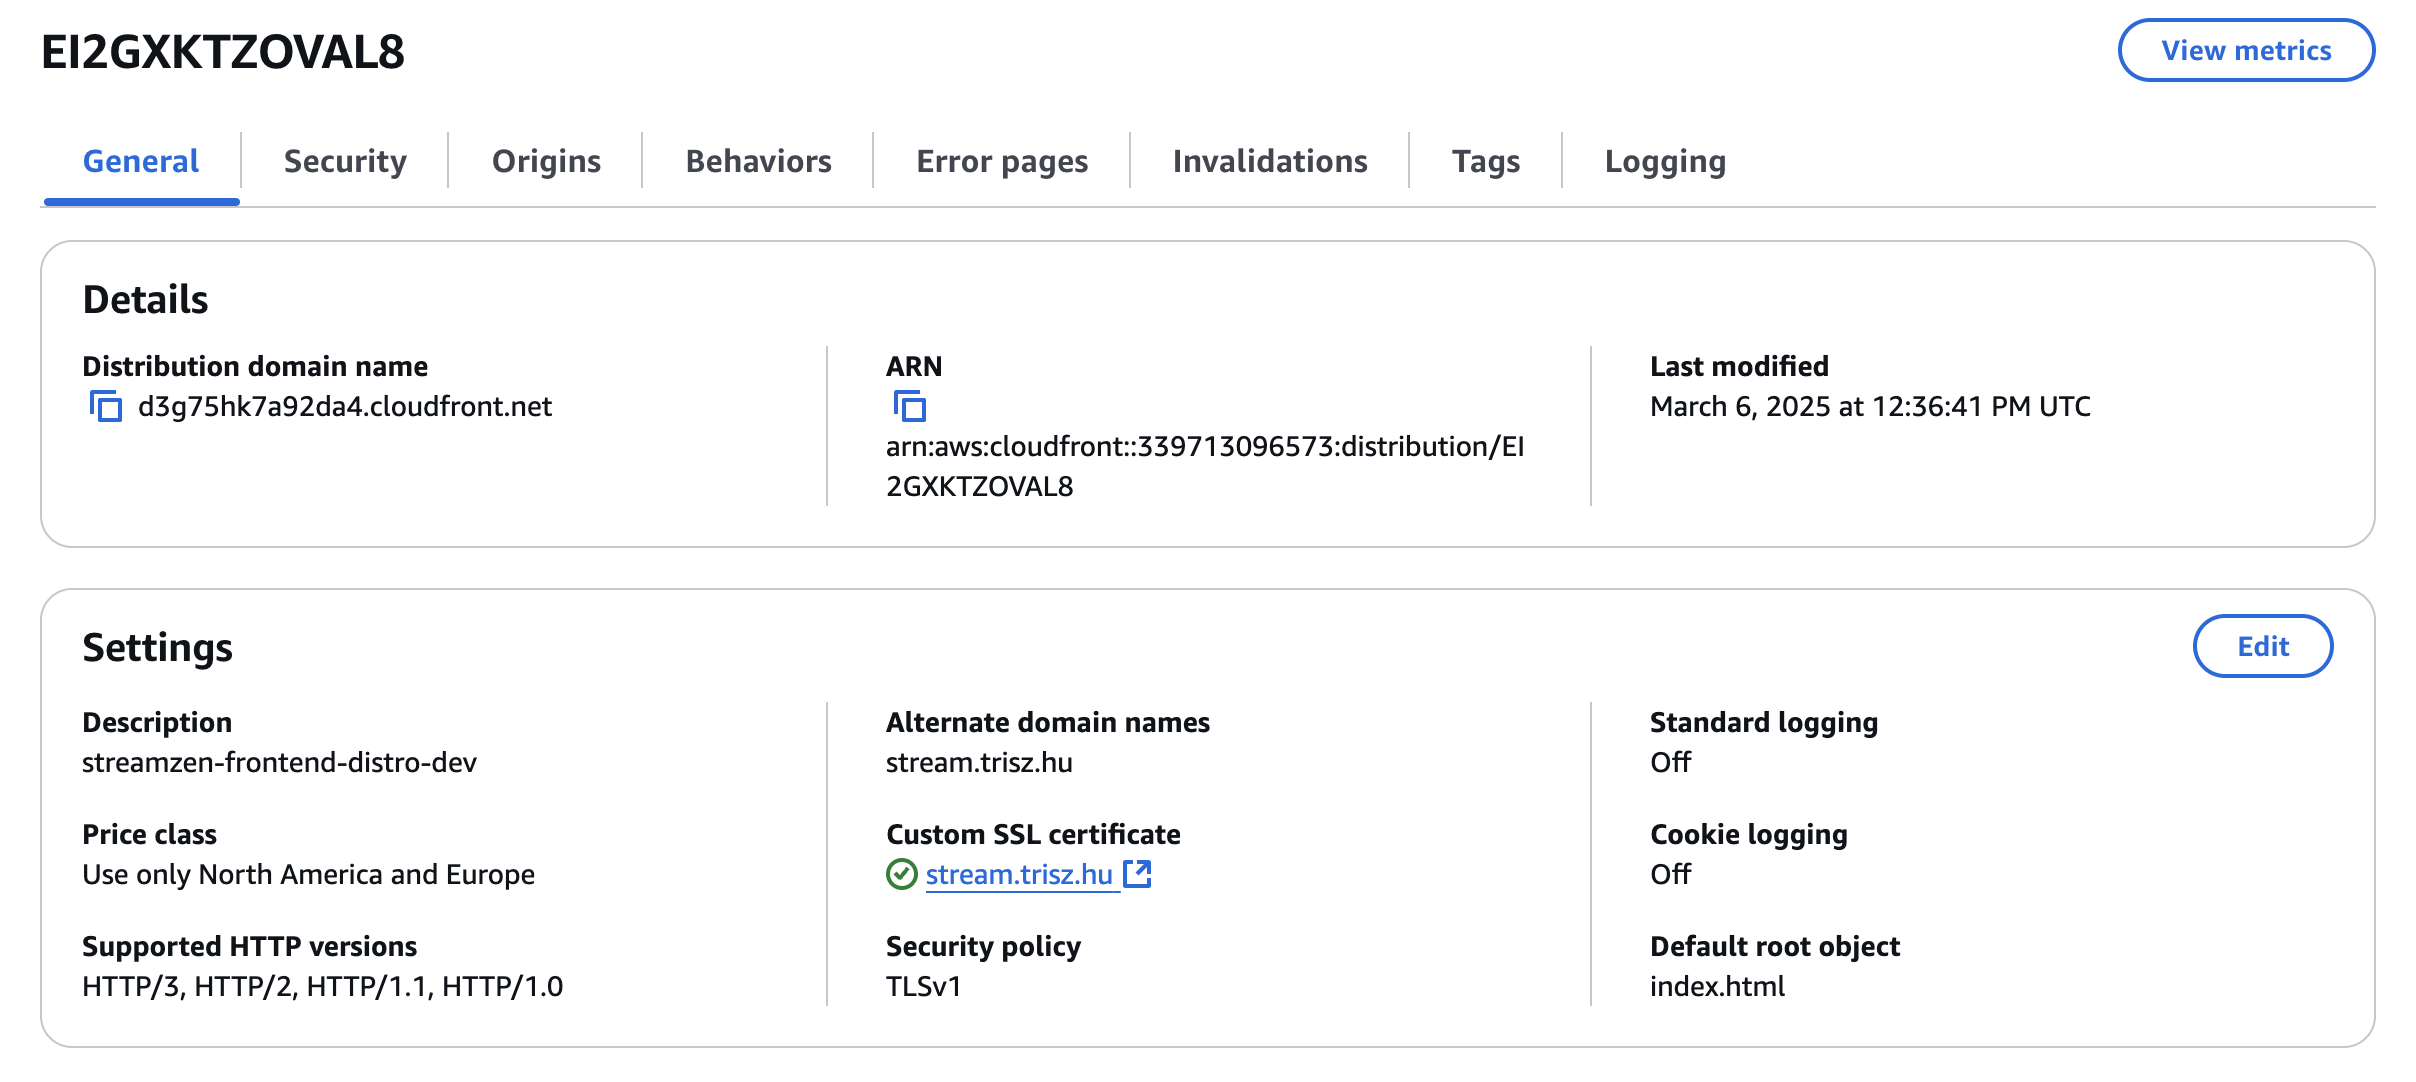
\includegraphics[width=150mm, keepaspectratio]{figures/distro_main.png}
  \caption{Képernyőkép a disztribúció alapvető beállításairól az AWS-konzolon.}
  \label{fig:distro}
\end{figure}

A Cloudfront disztribúcióhoz hozzácsatoltam egy WAF ACL-t, amely a webalkalmazás szintű tűzfal szerepét tölti be. Minden kérést ez a Layer 7 rétegbeli logika szűri meg. Mivel nem volt élő forgalomra készítve az alkalmazás, így egy egyszerű AWS menedzselte szabályt tettem csak rá a WAF-ra demonstrációképp, amely megvizsgálja a kérést, hogy tartalmaz-e SQL injection támadást vagy egyéb megszokott webalkalmazásokra jellemző ilyen jellegű támadást (pl.: ismert kihasználható URI-útvonalak, Java webalkalmazásokra jellemző exploitok) -- a szabálycsoportot név szerint \verb|AWSManagedRulesKnownBadInputsRuleSet| név alatt tartja számon az AWS WAF.

\begin{figure}[ht]
  \centering
  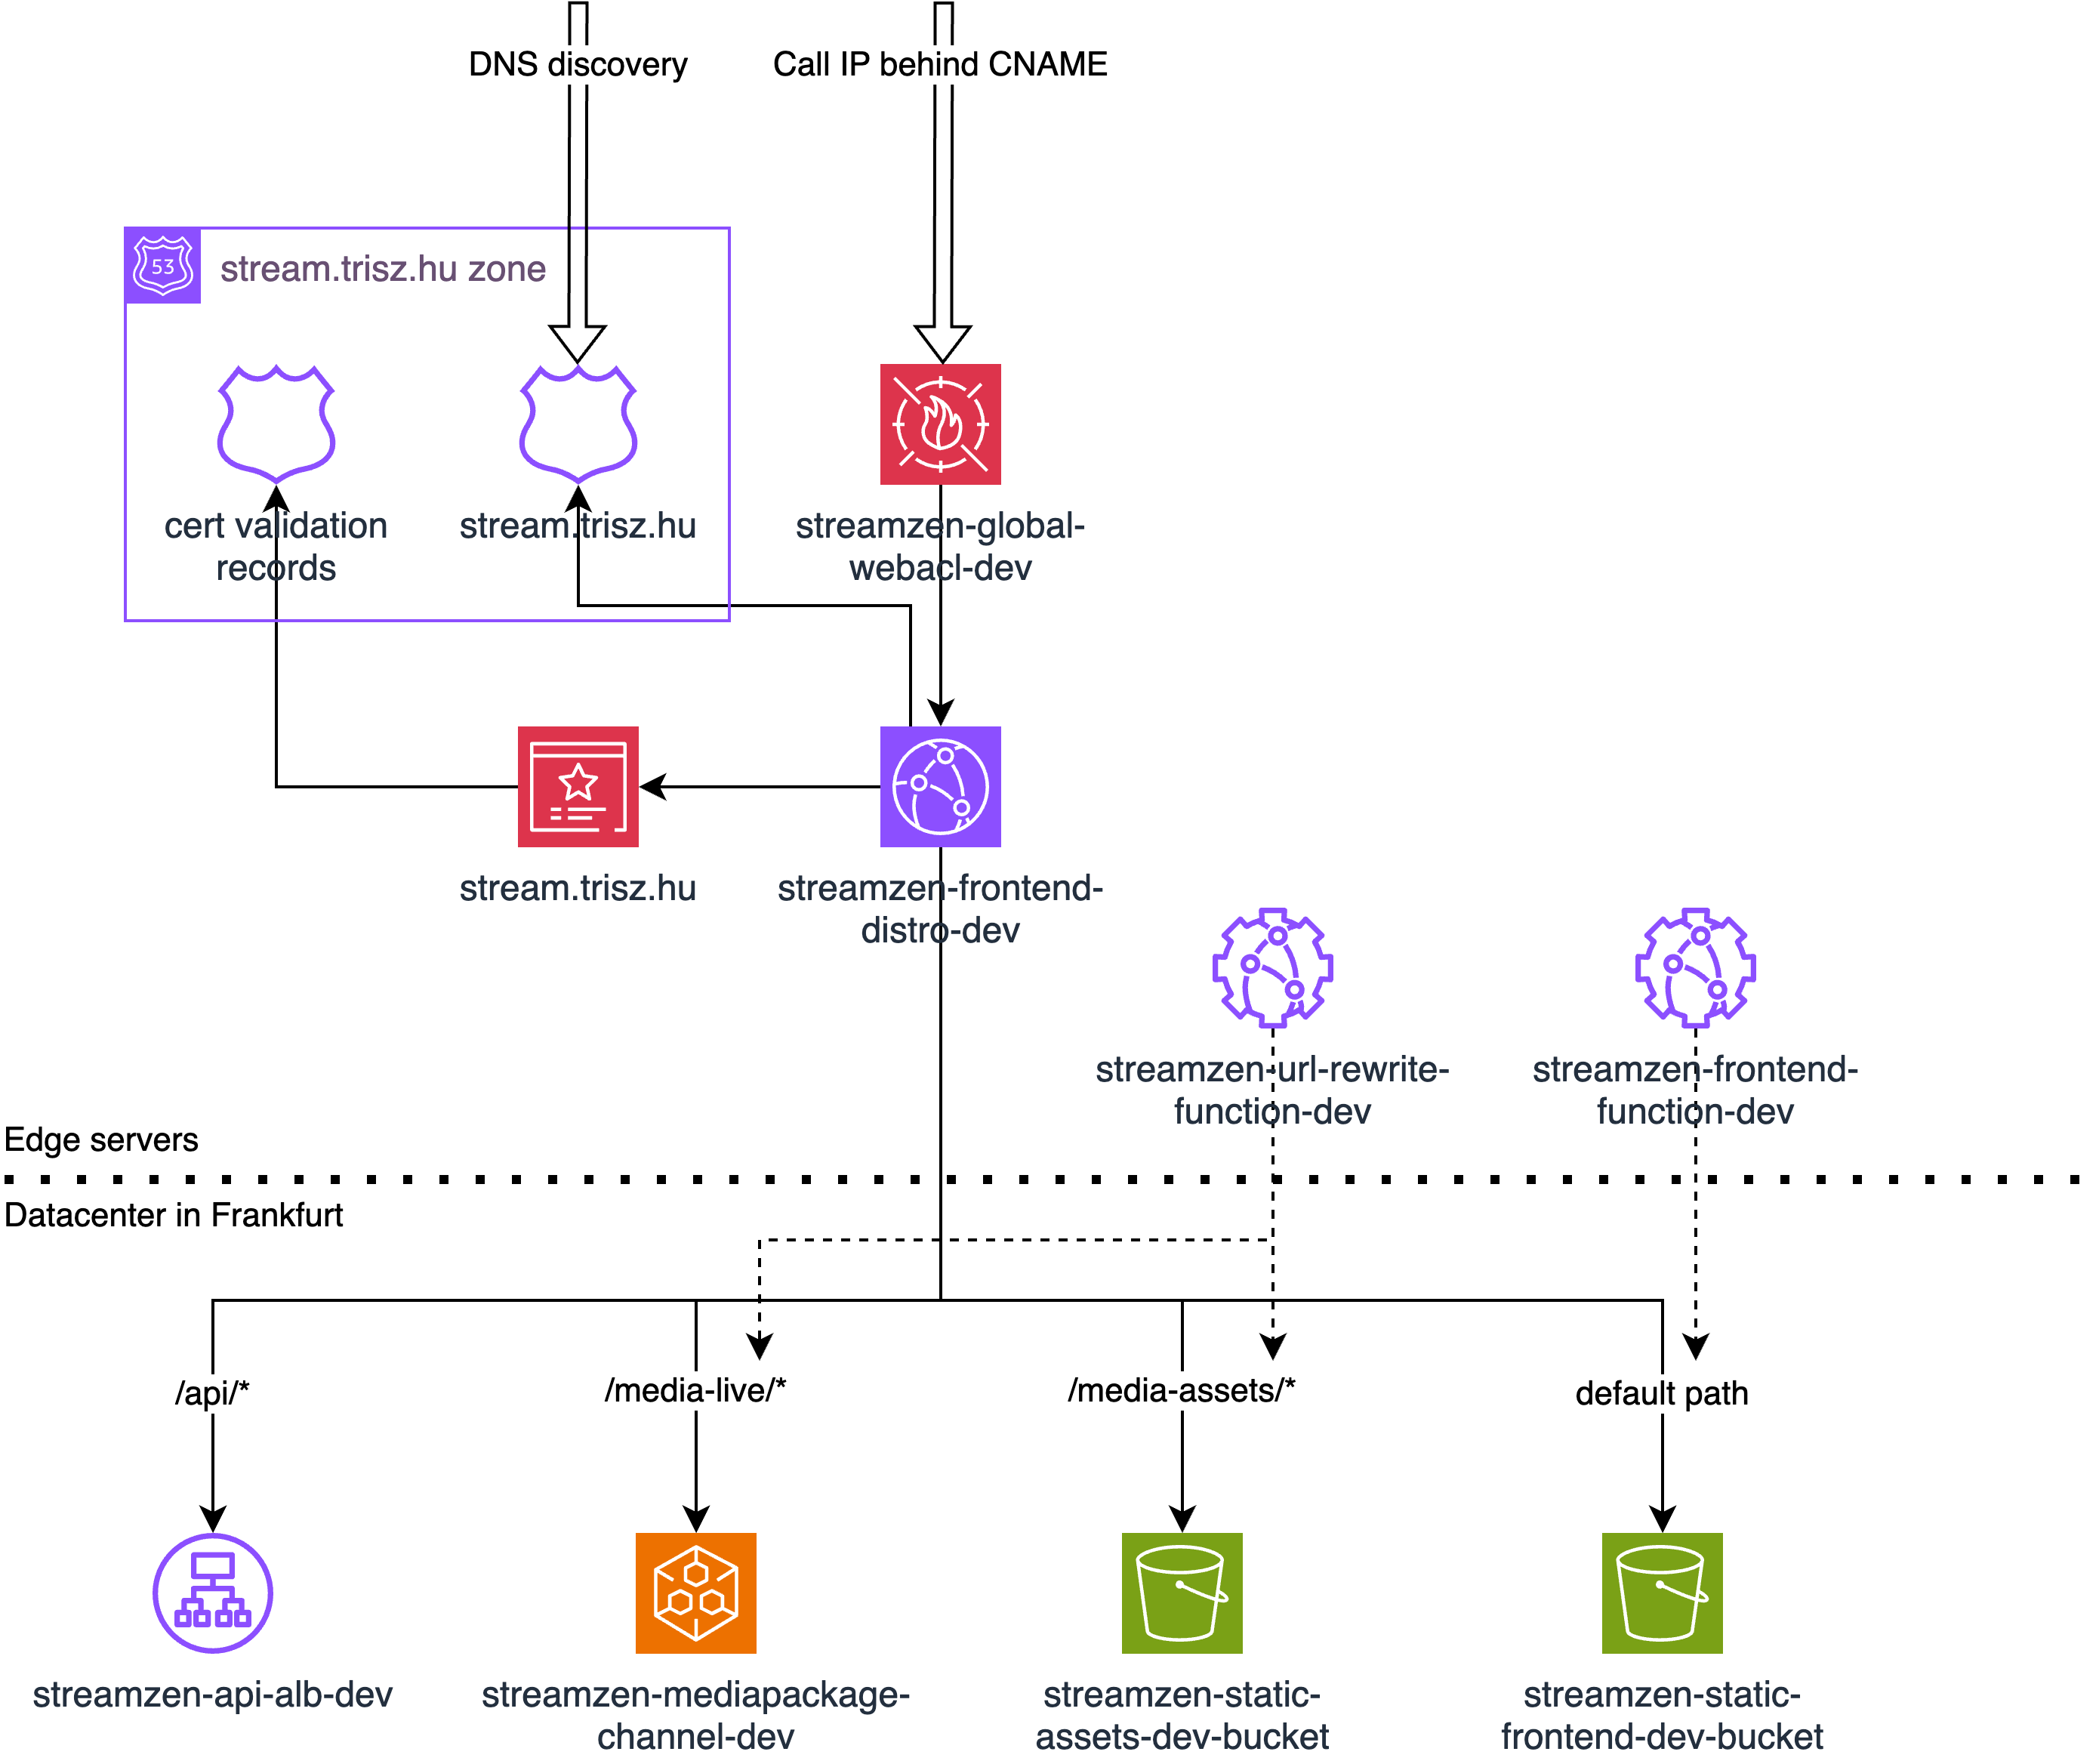
\includegraphics[width=150mm, keepaspectratio]{figures/dipterv_client.png}
  \caption{A kliensoldali architektúra részletezésebben.}
  \label{fig:client}
\end{figure}

Az edge-en kerül kiértékelésre a kapott kérés útvonala (angolul \emph{path}) alapján az, hogy melyik origin felé kell továbbítsa a disztribúció a kérést. A \refstruc{fig:client} adatközpont (angolul \emph{datacenter}) felőli oldalán láthatóak a nyilak végén, hogy milyen útvonalak alapján kerül a kérés melyik originhez. A kiértékelés során a disztribúció figyelembe veszi a szabályok sorrendjét, az szabályokban definiált útvonalmintákra mintaillesztés történik, és ha kapott útvonal illeszkedik a sorban következő mintára, ott véget és a kiértékelés. A disztribúcióhoz tartozó originok közül a legfontosabb a statikus weboldal, amely az S3-vödörben található, ez lett az alapértelmezett útvonal, ahova a kérések mennek, amennyiben egyik előbbi útvonalmintára se illeszkedik a kérésben található útvonal.

A Cloudfront biztosítja, hogy kis számításigényű logikát tudjuk még az edge rétegében futtatni a kéréseken, erre Cloudfront Function függvényeket alkalmaztam a MediaPackage csatorna előtt és a VOD-okat kiszolgáló S3 bucket (\verb|streamzen-static-assets-dev-bucket|) előtt. Ez a \verb|streamzen-url-rewrite-function| nevű kis függvény egy \verb|url-rewrite.js| nevű fájlt futtat (\ref{lst:urlrewrite}. kódrészlet). A függvény a kérés URI-ját vizsgálja, és ha a kérés a \verb|/media-assets/| vagy \verb|/media-live/| prefixekkel kezdődik, akkor eltávolítja ezeket a prefixeket, és a kérés így megtisztított URI-ját továbbítja a konkrét origin felé.

\begin{minipage}{0.92\textwidth}
  \begin{lstlisting}[
  caption=url-rewrite.js fájl tartalma.,
  label=lst:urlrewrite,
  basicstyle=\fontsize{10}{12}\ttfamily,
  style=js,
]
function handler(event) {
  const request = event.request;
  ["/media-assets/", "/media-live/"].forEach((prefix) => {
    request.uri = request.uri.replace(prefix, "/");
  });
  return request;
}
\end{lstlisting}
\end{minipage}

A backend \verb|/api| útvonalon keresztül elérhető, a Cloudfrontból ide egy VPC Origin típusú módon lehet továbbítani a kérést, ezzel leegyszerűsítve a kérések hálózati biztonsági kezelését. Ennek az originnek a cache behaviorje nem igényli, hogy lehagyjuk a Host headert, ugyanis az ALB mögötte akár fel tudja használni a forgalomirányításhoz. A többi origin esetén a Host headert le kell hagyni a kérésekről (működésük ezt igényli az AWS dokumentáció alapján dolgozva), ezért is került használatra ezeken az útvonalakon a \verb|Managed-AllViewerExceptHostHeader| nevű Origin Request Policy, azaz ez a kéréseket minden headerrel továbbítja, kivéve a Host headert. A behaviorok mindegyikénél beállítottam, hogyha HTTP-vel jönne a kérés, akkor dobja vissza a kliens felé, hogy kezdje újra HTTPS alapon a kérést. A cachelési szabályzásokat nem volt célom túlbonyolítani, így egyszerű menedzselt optimalizált cache policy-t használtam, amely a legjobban optimalizálja a cachelési időt. Az API-n kívül a többinél be kellett állítsam, hogy az alap CORS-fejléceket (\verb|Managed-CORSHeaders|) visszaküldje a kliens felé a disztribúció, hogy a böngésző ne blokkolja a válaszokat. Az API esetében maga a NestJS alkalmazás kezeli ezt. Ezen beállításokat mutatja be a \refstruc{fig:behav} is.

\begin{figure}[ht]
  \centering
  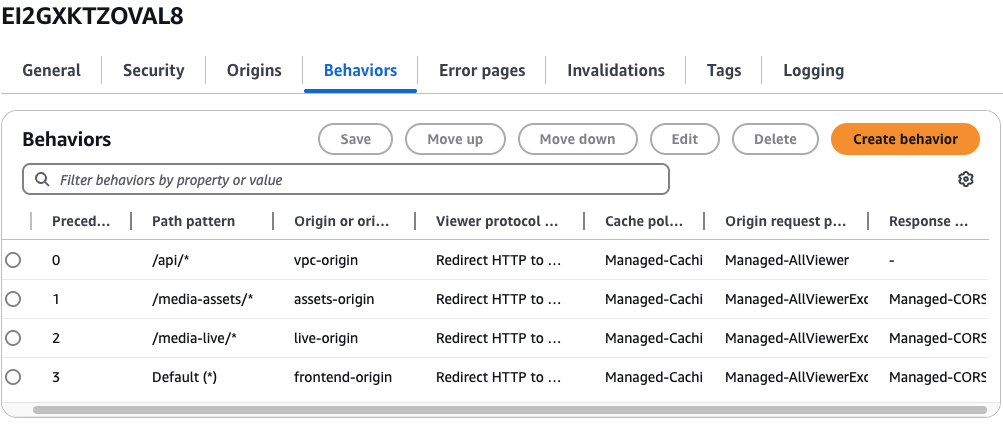
\includegraphics[width=150mm, keepaspectratio]{figures/distro_behav.png}
  \caption{Képernyőkép a különböző útvonalakra illesztett cache behavior-ökről.}
  \label{fig:behav}
\end{figure}

A VPC Origin típusú origin a Cloudfront disztribúcióban egy Amazon VPC-n belüli erőforrást jelent -- a mi esetünkben ez az ALB-példányunk --, amelyet a Cloudfront közvetlenül elérhet. Nem működik \emph{cross-account} módon, tehát amennyiben a célpont egy másik AWS-fiókban helyezkedne el. Az origin a VPC-n belül található, és elsősorban privát alhálózaton, security groupokkal van védve hálózati szinten. A VPC Origin típusú origin használata lehetővé teszi, hogy a Cloudfront közvetlenül kommunikáljon az erőforrással, anélkül hogy nyilvános doménnevet kelljen rendelni hozzá. Ezzel megspórolhatjuk az ALB Internet Gatewayre való kötését, az ALB számára domén bejegyzését, valamint SSL-tanúsítvány felvételét annak, a TLS-kapcsolat is terminálhat a Cloudfront disztribúcióban, házon belül már elég HTTP-alapon forgalmazni komponensek között.

Az S3-vödrök publikus elérését teljes blokkolásra állítottam (\refstruc{fig:s3policy}). Úgy tettem őket elérhetővé a Cloudfront disztribúció számára, hogy egy-egy bucket policy-t csatoltam hozzájuk, amely az S3 originre egyedi, arra csatolt Origin Access Controllal (OAC)\cite{oac} együtt lehetővé teszi, hogy csupán az az AWS-beli principal -- azaz a mi disztribúciónk -- kapjon csupán az objektumolvasásokra hozzáférést, amelynek a megadott Amazon Resource Number (ARN) azonosítója van. Az ábrán megadott \verb|AWS:SourceArn| a \verb|streamzen-frontend-distro-dev| disztribúció ARN-je. A fent gyakorolt beállítás is biztosítja az IT-biztonságban is elterjedt és az AWS által is ösztönzött \emph{"principle of least privilege (PoLP)"} elvét.

\begin{figure}[ht]
  \centering
  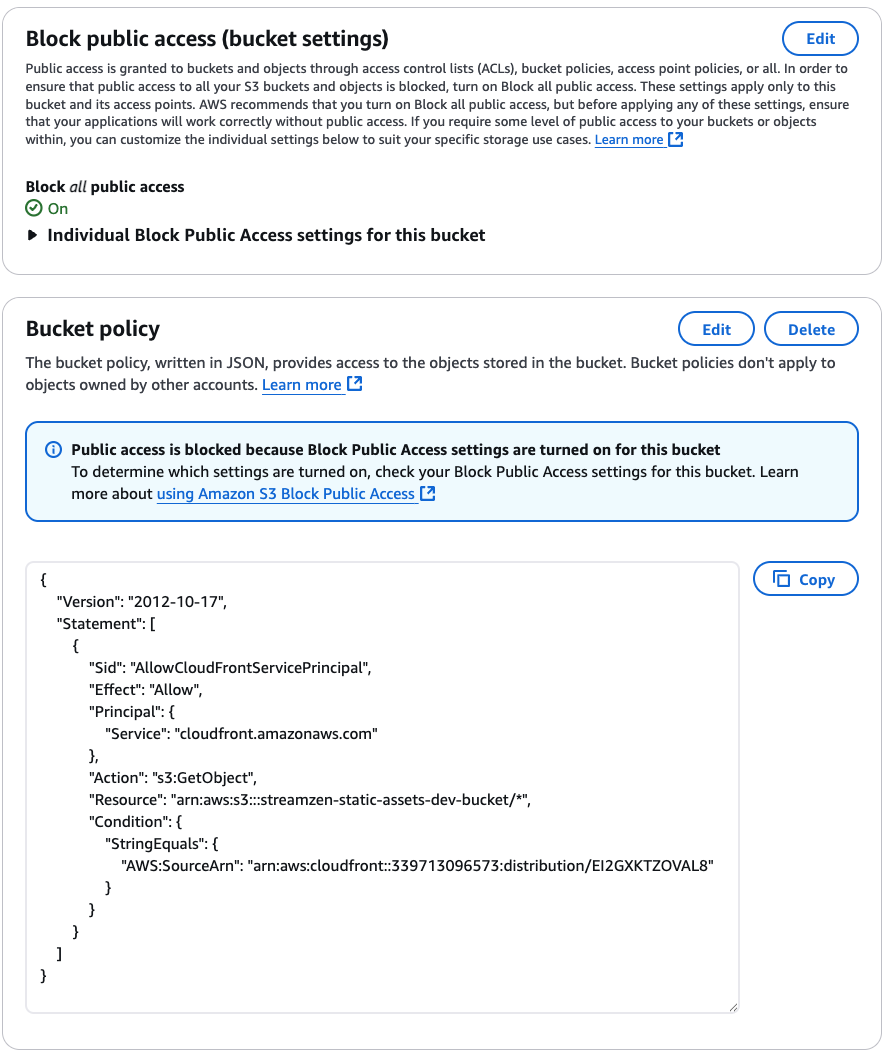
\includegraphics[width=150mm, keepaspectratio]{figures/distro_s3policy.png}
  \caption{Képernyőkép a vödrök hozzáférési beállításairól.}
  \label{fig:s3policy}
\end{figure}

A MediaPackage-csatorna védettségét pedig a publikált HLS-végpontra beállított \emph{CDN Authorization}\cite{cdnauth} segítségével biztosítottam, amely a Cloudfront disztribúciótól érkező kérésekben a \verb|X-MediaPackage-CDNIdentifier| headerben várja el egy titkos kulcs-érték párból az értéket. Ezt a headert a disztribúció felkonfigurálásakor a megfelelő originra rátettem. A MediaPackage-csatorna HLS-végpontjának hozzáférési beállításait, a felhasznált Secret Managerből származó kulcs-érték pár ARN-jét, és az azt elérő IAM-szerep ARN-jét a \refstruc{fig:mediapack} mutatja be.

\begin{figure}[ht]
  \centering
  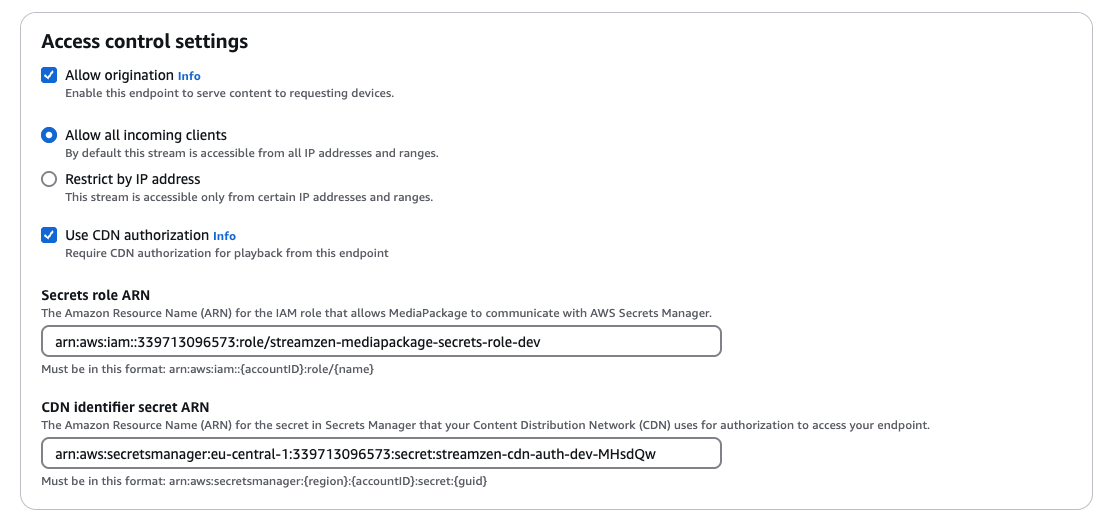
\includegraphics[width=150mm, keepaspectratio]{figures/distro_mediapack.png}
  \caption{Képernyőkép a MediaPackage-csatornabeli HLS-végpont hozzáférési beállításairól.}
  \label{fig:mediapack}
\end{figure}

\section{A statikus weboldal}

A statikus weboldal HTML-, JavaScript- és CSS-fájlokból, valamint a weboldal statikus tartalmát képező médiafájlokból (képek, betűtípusok) tevődik össze. Ezek összeállításához a React keretrendszerben írt SPA-alkalmazásokat is jól kezelő Vite.js eszközt használtam, amely a React alkalmazásokat egyetlen kiindulási \verb|index.html| HTML-fájlba csomagolja, és a készülő JavaScript-kódot is optimalizálja. A Vite.js eszköz a fejlesztési környezetben gyorsítótárazza a fájlokat, így gyorsabbá téve a fejlesztést, míg a gyártási környezetben (angolul \emph{in production}) optimalizálja azokat, hogy a lehető legkisebb méretűek legyenek.

Korábban bemutatásra került két különböző Cloudfront Function függvény, amelyek az S3-vödrök elérése előtt futnak minden kérésen. Ezek közül a statikus weboldal előtti függvény (\ref{lst:frontend}. kódrészlet) csupán arra hivatott, hogy a kéréseknél az egyes prefixekkel kezdődő kéréseket átirányítsa az alapértelmezett \verb|/| útvonalra. Ezekre azért volt szükség, hogy a statikus oldal által kezelt útvonalak mind a CDN-re való belépés után az alapértelmezett útvonalon elérhető \verb|index.html|-re oldódjanak fel, hiszen az indexoldalon behivatkozott JavaScriptből pedig majd a betöltés után a React Router megfelelően kezeli le a böngészőben az eredetileg kért útvonalat. Ez a megoldás természetesen magával vonzza azt az igényt, hogy akármikor ha új aloldalt vezetünk be, akkor a Cloudfront Function függvényben ezt a prefixet hozzá kell adnunk a \verb|spaInternalRoutingPrefixes| tömbhöz, amely a kód elején található.

\begin{minipage}{0.92\textwidth}
  \begin{lstlisting}[
  caption=frontend-request-default.js fájl tartalma.,
  label=lst:frontend,
  style=js,
  basicstyle=\fontsize{10}{12}\ttfamily
]
const spaInternalRoutingPrefixes = ["/videos", "/live", "/events", "/members", 
  "/courses", "/about", "/studio", "/login"];
function handler(event) {
  const request = event.request;
  if (spaInternalRoutingPrefixes.some((pref) => request.uri.startsWith(pref))) {
    request.uri = "/";
  }
  return request;
}
\end{lstlisting}
\end{minipage}

\subsection{A React alkalmazás fejlesztése}

TODO: ejlesztés részletei. Nem annyira lényeges most ebben a dolgozatban, de néhány szép kihívást jelentő kidolgozott form és egyebeket be lehet itt mutatni.

\subsection{A weboldal telepítésének CI/CD folyamata}

TODO: GitHub Actions a smoke tesztekre, workflowk, a deploymentek. Értsd itt: S3 telepítés.

\section{Média erőforrások objektumtárolói}

TODO: Hogy lettek felkonfigurálva és miért az egyes S3 bucket-ok (bucket policy, CORS policy).

\section{A MediaLive és MediaPackage bekötése}

TODO: Az Elemental stack részeinek felkonfigurálása, a MediaLive channel és a MediaPackage channel felépítése, a MediaPackage endpoint konfigurálása. Miként kerül kiszolgálásra, melyiket mire használom. OBS bekötésének módja.

\chapter{Szerver oldali folyamatok implementációi}

\section{A virtuális privát felhő komponensei}

A VPC-beli (Virtual Private Cloud) subnetek, a security groupok, route táblák. A biztonság vizsgálata.

\section{A Node.js alkalmazás fejlesztése}

Fejlesztés részletei. Kitérve arra, hogy miképp könnyíti a munkát a Prisma, milyen egyéb szolgáltatások kerültek be, mi a felépítése a reponak, miért választottam ezt a stacket. S3 bucketba való mentése a videónak egy érdekes rész. Itt lehet szó az adatbázisbeli entitásokról is.

\section{A konténerizált környezet}

Leírás, hogy miért választottam a konténerizált környezetet, a konténerizálás előnyeit, hátrányait. Hogy használható ki a legjobban a konténerizáció az Application Load Balancer-rel együtt. Miképp kapcsoltam ezt a kettőt össze (ECS service, ALB).

\subsection{A Node.js szerveralkalmazás ECS-en}

Az ECS orkesztrációs toolsetjének kialakítása, a konténer rétegződés felépítése ECS-ben, a konténer registry (ECR) bekötése. Környezeti változók, portok, ALB-re való kötése. Miből állt a dockerizálás nekem (Dockerfile, registry, image build, push, networking).

Milyen IAM role-okat kellett feltenni rá, mikkel kommunikál kifelé, mi indokolta, hogy publikus subnetbe kerüljön. Hogy hív meg más külső rácsatlakozó erőforrásokat (S3 bucket, RDS instance, Lambda függvény, MediaLive channel).

\subsection{A szerveralkalmazás CI/CD folyamatai}

GitHub Actions a smoke tesztre, a deploymentre: Docker build és ECR-be telepítés.

\section{Elemental MediaConvert felhasználása}

Az Elemental MediaConvert API használata a Lambdából, illetve hogy hogy hívódik meg a Lambda, milyen triggerrel, milyen környezeti változókkal, milyen IAM role-al. Hogy kellett felkonfigurálni a MediaConvert job, hogy kellett magát a Lambdát felkonfigolni, hogy tudja is hívni.

\chapter{Rétegeken átívelő szolgáltatások implementációja}

Ebben a fejezetben kerül kifejtésre az implementációja olyan szolgáltatásainak az alkalmazásnak, amelyek a kliens és szerver rétegén átívelnek, és külön-külön nem lenne érdemes bemutatni őket.

\section{Single Sign-On (SSO) integrációja}

A videók feltöltésére azok jogosultak, akik a stúdióba be tudnak lépni a \verb|/studio| aloldalon, a bejelentkeztetéshez pedig a kari hallgatói közösségünk által nyílt forráskóddal fejlesztett AuthSCH nevű Single Sign-On (SSO) rendszert integráltam be a weboldalba,  ennek az esszenciális tokenkezelési implementációs részeit a backendre bíztam, a kliensoldal csupán a megfelelő útvonalakra irányításért felel.

A \ref{lst:authCtx}. kódrészlet mutatja be a React-alkalmazásban használt \verb|AuthCtx| nevű kontextust, amely JSON Web Tokeneket (JWT) használ a bejelentkeztetés során a felhasználói adatok biztonságos és állapotmentes átpasszolására. A \verb|useMe| nevű hook az AuthSCH SSO API-ját használja a bejelentkezett felhasználó adatainak lekérdezésére, amelyet a \verb|/api/me| végponton keresztül érhetünk el. A \verb|AuthProvider| komponens biztosítja a kontextust az alkalmazás többi részének, és kezeli a bejelentkezést és kijelentkezést.

\begin{minipage}{0.92\textwidth}
  \begin{lstlisting}[
  caption=src/hooks/auth-context.tsx fájl tartalma.,
  label=lst:authCtx,
  style=js,
  basicstyle=\fontsize{10}{12}\ttfamily
]
import { createContext, PropsWithChildren } from "react"
import { useMe } from "./use-me.hook"

type AuthCtxType = {
  authenticated: boolean
  isLoading: boolean
  login: () => void
  logout: () => void
}
export const AuthCtx = createContext<AuthCtxType | undefined>(undefined)

export function AuthProvider({ children }: PropsWithChildren) {
  const { data, isLoading } = useMe()
  const onLogin = async () => {
    window.location.href = import.meta.env.VITE_BACKEND_URL+"/auth/login"
  }
  const onLogout = async () => {
    window.location.href = import.meta.env.VITE_BACKEND_URL+"/auth/logout"
  }
  const value = {
    authenticated: !!data,
    isLoading,
    login: onLogin,
    logout: onLogout,
  }
  return <AuthCtx.Provider value={value}>{children}</AuthCtx.Provider>
}
\end{lstlisting}
\end{minipage}
\chapter{Összegzés}

TODO: Tanulságok, a rendszer működésének és fejlesztési élmények értékelése. Média streaming jövője saját meglátások szerint.

\section{Továbbfejlesztés lehetőségei}

TODO: Min lehetne javítani, mikroszolgáltatásos architektúra stb.

\subsection{Vendor lock-in jelensége}

TODO: Miként befolyásolja egy üzlet működését a vendor lock-in, és hogyan lehet ezt kezelni. Miképp lehetne a jövőben a vendor lock-in-t csökkenteni ebben a rendszerben. S3 helyett Ceph, konténert kiemelni, akár K8s-re felkészíteni, hogy ne ECS-től függjön.


% %----------------------------------------------------------------------------
\chapter*{\koszonetnyilvanitas}\addcontentsline{toc}{chapter}{\koszonetnyilvanitas}
%----------------------------------------------------------------------------

Ez nem kötelező, akár törölhető is. Ha a szerző szükségét érzi, itt lehet köszönetet nyilvánítani azoknak, akik hozzájárultak munkájukkal ahhoz, hogy a hallgató a szakdolgozatban vagy diplomamunkában leírt feladatokat sikeresen elvégezze. A konzulensnek való köszönetnyilvánítás sem kötelező, a konzulensnek hivatalosan is dolga, hogy a hallgatót konzultálja.
%\listoffigures\addcontentsline{toc}{chapter}{\listfigurename}
%\listoftables\addcontentsline{toc}{chapter}{\listtablename}
\addcontentsline{toc}{chapter}{\bibname}
\bibliography{bib/mybib}
% %----------------------------------------------------------------------------
\appendix
%----------------------------------------------------------------------------
\chapter*{\fuggelek}\addcontentsline{toc}{chapter}{\fuggelek}
\setcounter{chapter}{\appendixnumber}
%\setcounter{equation}{0} % a fofejezet-szamlalo az angol ABC 6. betuje (F) lesz
\numberwithin{equation}{section}
\numberwithin{figure}{section}
\numberwithin{lstlisting}{section}
%\numberwithin{tabular}{section}

%----------------------------------------------------------------------------
\section{A TeXstudio felülete}
%----------------------------------------------------------------------------
\begin{figure}[!ht]
\centering
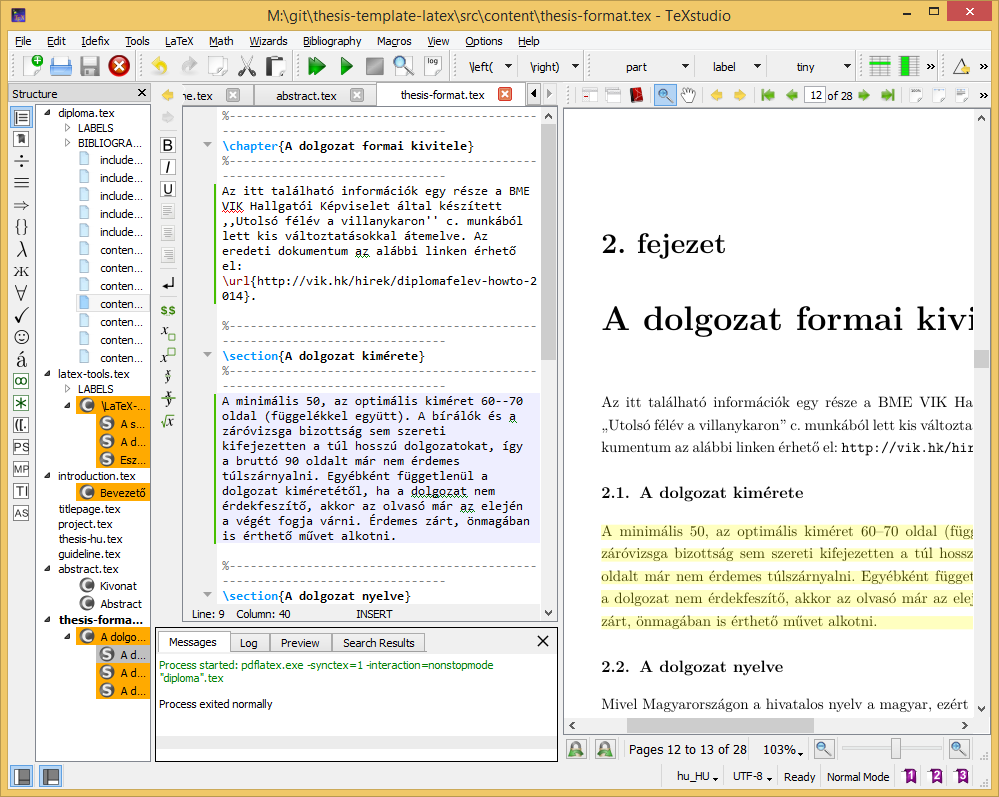
\includegraphics[width=150mm, keepaspectratio]{figures/TeXstudio.png}
\caption{A TeXstudio \LaTeX-szerkesztő.} 
\end{figure}

%----------------------------------------------------------------------------
\clearpage\section{Válasz az ,,Élet, a világmindenség, meg minden'' kérdésére}
%----------------------------------------------------------------------------
A Pitagorasz-tételből levezetve
\begin{align}
c^2=a^2+b^2=42.
\end{align}
A Faraday-indukciós törvényből levezetve
\begin{align}
\rot E=-\frac{dB}{dt}\hspace{1cm}\longrightarrow \hspace{1cm}
U_i=\oint\limits_\mathbf{L}{\mathbf{E}\mathbf{dl}}=-\frac{d}{dt}\int\limits_A{\mathbf{B}\mathbf{da}}=42.
\end{align}


\label{page:last}
\end{document}
